\documentclass{sigplan-proc}
%\documentclass[10pt]{sigplanconf}

\usepackage{booktabs}
\usepackage{colortbl}
\usepackage{tabularx}
\usepackage{multirow}
\usepackage{color}
\usepackage{xspace}
\usepackage{hyperref}    % Creates hyperlinks from ref/cite 
\hypersetup{pdfstartview=FitH}
\usepackage{graphicx}    % For importing graphics
\usepackage{url}         %
\usepackage{verbatim}
\usepackage{amssymb}
\usepackage{amsmath}
\relpenalty=9999
\binoppenalty=9999

\newcommand{\2}{\;\;}
\newcommand{\5}{\;\;\;\;\;}
\newcommand{\brk}{\textbf{\small{$^\wedge$}}}
\newcommand{\CEU}{\textsc{C\'{e}u}}
\newcommand{\nesc}{\emph{nesC}}
\newcommand{\code}[1] {{\small{\texttt{#1}}}}
\newcommand{\Code}[1] {\texttt{#1}}

\begin{document}

%\conferenceinfo{Onward! '12}{date, City.}
%\copyrightyear{2012}
%\copyrightdata{[to be supplied]}

\title{\CEU{}: Embedded, Safe, and Reactive Programming}

\begin{comment}
\authorinfo{Francisco Sant'Anna, Noemi Rodriguez, Roberto Ierusalimschy}
        {Departamento de Inform\'atica --- PUC-Rio, Brasil}
        {\{fsantanna,noemi,roberto\}@inf.puc-rio.br}

\authorinfo{Name1}
           {Affiliation1}
           {Email1}
\authorinfo{Name2\and Name3}
           {Affiliation2/3}
           {Email2/3}

===============================================================================
TODO:
===============================================================================

- simulation langs
- sol?

- future work
    - parallel
    - processes in the OS (output events)
    - dynamic support
    - better DFA

- Demo Mario
    - usar dataflow

- ver trabalhos de todos do comite
     Bjorn Nathan Freeman Benson:
        Experience in developing the urbanSim system: tools and processes
        An incremental constraint solver
        Constraint hierarchies
        Kaleidoscope: mixing objects, constraints, and imperative programming

    Caitlin Sadowski
        SingleTrack: A dynamic determinism checker for multithreaded programs
        Cooperative reasoning for preemptive execution
        Practical parallel and concurrent programming
        Heuristic evaluation of programming language features

    Derek:
        Compact Java binaries for embedded systems 

    Tom van Cutsem:
        Ambient-oriented programming in ambienttalk
        Ambienttalk: Object-oriented event-driven programming in mobile ad hoc networks

- concurrent returns, falar algo no exemplo do ship

- loop break concurrent
  Note that loops with nested parallel statements may escape from different 
  trails (through the \code{break} statement).
  The behavior for escaping a loop is similar to a \code{par/or} rejoin, being 
  handled the same way.

- impl internal events?

- medir o overhead de tamanho e execucao de trails

- nondet C pointers \& arrays

- Esterel: fazer convesao p/ mostrar como ceu eh equiv. (e o oposto?)

\end{comment}

\maketitle

\begin{abstract}

\CEU{} is a programming language that unifies the features found in dataflow 
and imperative synchronous reactive languages, offering a high-level and safe 
alternative to event-driven and multithreaded systems for embedded systems.

\CEU{} supports concurrent lines of execution that run in time steps and are 
allowed to share variables.
However, the synchronous and static nature of \CEU{} enables a compile time 
analysis that can enforce deterministic and memory-safe programs.

\CEU{} also introduces first-class support for ``wall-clock'' time (i.e. time 
from the real world), and offers seamless integration with $C$ and simulation 
of programs in the language itself.

The \CEU{} compiler generates single-threaded code comparable to handcrafted 
$C$ programs in terms of size and portability.
\end{abstract}

\category{D.3}{Programming Languages}{General}

\terms{Design, Languages}

\keywords{Esterel, Concurrency, GALS, Synchronous, Determinism, Dataflow, 
Static Analysis, Embedded Systems, Wireless Sensor Networks}

\section{Introduction}
\label{sec:intro}

Embedded systems combine hardware, software, and possibly mechanical devices to 
perform a specific dedicated task.
They differ from general-purpose systems, which are designed with flexibility 
in mind and encompass a multitude of applications in a single system.
Examples of embedded systems range from simple MP3 players to complex 
fly-by-wire avionic systems.
Usually they have a very low tolerance to faults, are constrained in memory and 
processing, and must conform with real-time requirements.

Embedded systems are essentially reactive as they interact permanently with the 
surrounding environment through input and output devices (e.g. buttons, timers, 
touch displays, etc.).

% TODO: ref
Software for embedded systems is usually developed in $C$, and the addition of 
a real-time operating system may extend it with preemptive and/or cooperative 
multithreading (\emph{MT}).
However, concurrency in $C$ requires a low-level exercise related to the life 
cycle of activities (i.e. creating, starting, and destroying threads), besides 
extra efforts for explicit scheduling (in cooperative \emph{MT}) and manual
synchronization (in preemptive \emph{MT}).
Furthermore, these models lack safety warranties, given that 
cooperative \emph{MT} is susceptible to unbounded execution, while 
preemptive \emph{MT} is subject to race conditions and deadlocks.

An established alternative to $C$ in the field of safety-critical embedded 
systems are reactive synchronous languages \cite{rp.twelve}.
Two major styles of synchronous languages have evolved:
in the \emph{control}--\emph{imperative} style (e.g. Esterel 
\cite{esterel.design}), programs are structured with control flow primitives, 
such as parallelism, repetition, and preemption;
in the \emph{dataflow}--\emph{declarative} style (e.g. Lustre 
\cite{lustre.ieee91}), programs can be seen as graphs of values, in which a 
change to a value is propagated through its dependencies without explicit 
programming.

We believe that embedded systems programming can benefit from a new language 
that reconciles both reactive synchronous styles, while preserving typical $C$ 
features that programmers are familiarized, such as shared memory concurrency.

In this work, we present \CEU, a reactive language targeting embedded systems 
that unifies both imperative and dataflow synchronous programming styles.
\CEU{} is based on a small set of reactive control primitives similar in 
functionality to Esterel's \cite{esterel.design}.
On top of this kernel, \CEU{} provides disciplined side effects, which together 
with internal events enable dataflow capabilities to the language.

Besides offering a high-level reactive programming model, a primeval goal of 
\CEU{} is to ensure the correctness of programs through safety warranties.
\CEU{} relies on a compile-time analysis to detect unbounded loops and 
concurrent access to variables.
The static analysis precludes any dynamic support in the language, such as 
memory allocation, a call stack, and dynamic loading.
However, this trade-off seems to be favorable in the context of embedded 
systems, as dynamic features are discouraged due to resource limitations and 
safety requirements.

\CEU{} has an open source implementation%
\footnote{\url{http://www.ceu-lang.org}}
targeted at highly constrained embedded platforms, such as Arduino%
\footnote{\url{http://www.arduino.cc}}
and wireless sensor nodes (e.g. \emph{micaz}%
\footnote{\url{http://www.xbow.com}}).
The current memory footprint of the \CEU{} runtime is around 4Kbytes of ROM and 
100bytes of RAM on a 16 bits platform.

This paper is organized as follows.
In Section~\ref{sec:ceu}, we introduce \CEU: its synchronous execution model, 
parallel compositions, dataflow support, first class wall-clock time, 
integration with $C$, safety warranties, and asynchronous execution.
In Section~\ref{sec:demos}, we demonstrate the applicability of \CEU{} with 
three demo applications in different scenarios, exploring the programming style 
promoted by the language.
%In Section~\ref{sec:eval}, we provide a quantitative analysis of \CEU, 
%comparing the memory usage and responsiveness of \CEU{} with existing 
%languages for Wireless Sensor Networks.
In Section~\ref{sec:impl}, we discuss the implementation of \CEU.
In Section~\ref{sec:related}, we compare \CEU{} with common approaches for 
programming embedded systems.
In Section~\ref{sec:conclusion}, we make final remarks and conclude the paper.

\section{The Language \CEU}
\label{sec:ceu}

\CEU{} is a concurrent language in which multiple lines of execution---known as 
\emph{trails}---continuously react to input events from the environment.
%The fundamental concept in \CEU{} is that of \emph{events}.
Waiting for an event suspends the running trail until that event occurs.
The environment broadcasts an occurring event to all active trails, which share 
a single global time reference (the event itself).

%The \code{await} and \code{emit} primitives of \CEU{}, together with parallel 
%compositions, are at the core of the concurrent model of \CEU{}.
To illustrate the concurrent reactive nature of \CEU{}, the example in 
Figure~\ref{lst:ceu:1} executes three trails in parallel through the \code{par} 
statement.
The first and second trails wait for different events and change the value of a 
variable, notifying all changes to the third trail, which continuously shows 
the current value of the variable.
 
\begin{figure}[t]
\rule{8.5cm}{0.37pt}
{\small
\begin{verbatim}
 1:  input int Restart;     // an external event
 2:  internal void changed; // an internal event
 3:  int v = 0;             // a variable
 4:  par do
 5:     loop do             // 1st trail
 6:        await 1s;
 7:        v = v + 1;
 8:        emit changed;
 9:     end
10:  with
11:     loop do             // 2nd trail
12:        v = await Restart;
13:        emit changed;
14:     end
15:  with
16:     loop do             // 3rd trail
17:        await changed;
18:        _printf("v = %d\n", v);
19:     end
20:  end
\end{verbatim}
}
\caption{ A concurrent program in \CEU{}.
\label{lst:ceu:1}
}
\end{figure}

\begin{figure*}[t]
\centering
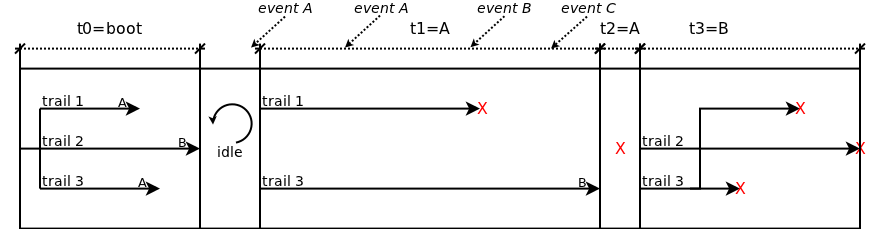
\includegraphics[scale=0.50]{reaction.png}
\caption{ A sequence of reaction chains for the program in 
Figure~\ref{lst:ceu:2}.
\label{fig:reaction}
}
\end{figure*}

Lines 1-3 declare the variables and events used in the program.
An event declaration must include the type of value the occurring event 
communicates.
For instance, the external event \code{Restart} carries integer values, while 
the internal event \code{changed} is a notify-only event, holding no values.
\footnote{\CEU{} uses uppercase letters to denote external events and lowercase 
letters to denote variables and internal events.}

The loop in the first trail (lines 5-9) waits for 1 second, increments variable 
\code{v}, and notifies changes through the \code{emit} statement (line 8).
The loop in the second trail (lines 11-14) resets \code{v} to the value of 
every occurrence of the input event \code{Restart} (line 12), and notifies 
these changes (line 13).
The loop in the third trail (lines 16-19) shows the value of \code{v} (line 18) 
whenever the event \code{change} is emitted (line 17).

\CEU{} uses a verbose notation with plenty of keywords, such as `\code{do}' and 
`\code{end}' to delimit blocks (instead of curly brackets).
Types, values, and expressions follow the same conventions of $C$.
Symbols defined externally in $C$, such as \code{printf} in the example, must 
be prefixed with an underscore to be used in \CEU{} programs (to be discussed 
in Section~\ref{sec:ceu:c}).

%The complete syntax of \CEU{} is available in Appendix~\ref{sec:syntax}.

\CEU{} is grounded on a precise definition of time as a discrete sequence of 
external input events:%
\footnote{We use the terms \emph{external input event}, \emph{external event}, 
and \emph{input event} interchangeably.}
a sequence because only a single input event is handled at a time; discrete 
because a complete reaction always executes in bounded time (to be discussed in 
Section~\ref{sec:ceu:bounded}).
The execution model for a \CEU{} program is as follows:

\begin{enumerate}
\setlength{\itemsep}{0pt}
\item The program initiates the ``boot reaction'' in a single trail.
\item Active trails execute until they await or terminate.
      This step is named a \emph{reaction chain}, and always runs in bounded 
      time.
\item If there are no remaining awaiting trails, the program terminates.
      Otherwise, the program goes idle and the environment takes control.
\item On the occurrence of a new external input event, the environment awakes 
      the trails awaiting that event.
      It then goes to step 2.
\end{enumerate}

When multiple trails are active at a time, \CEU{} does not specify the order in 
which they should execute.
The language runtime is allowed to serialize, interleave, or even parallelize 
their execution.

If a new external input event occurs while a reaction chain is running (step 
2), the environment enqueues it to run in the next reaction, because reaction 
chains must run to completion.

Every occuring event in \CEU{} has a corresponding reaction chain that spans 
for a bounded duration, even if there are no awaiting trails to react to the 
event.
In this case, an \emph{empty} reaction chain takes place, and the event is 
discarded.
% TODO: fleeting events

To illustrate the execution model of \CEU{}, Figure~\ref{fig:reaction} 
corresponds to an execution of the program in Figure~\ref{lst:ceu:2}.

\begin{figure}[t]
\rule{8.5cm}{0.37pt}
{\small
\begin{verbatim}
   input void A, B, C;
   par/and do   // trail 1
      ...   // a sequence of non-awaiting stmts
      await A;
      ...
   with         // trail 2
      ...
      await B;
      ...
   with         // trail 3
      ...
      await A;
      ...
      await B;
      par/and do
         ...
      with
         ...
      end
   end
\end{verbatim}
}
\caption{ An example of a program in \CEU{}.
\label{lst:ceu:2}
}
\end{figure}
The program starts in the ``boot'' reaction in a single trail that splits in 
three: \emph{trails~1} and \emph{3} execute and wait for the event $A$, while 
\emph{trail~2} waits for the event $B$.
Control next goes back to the scheduler, which remains idle until a new event 
occurs.
The \code{par/and} statements used in the example only terminate when all of 
its trails in parallel terminate (to be discussed in Section~\ref{sec:ceu:par}.

The occurrence of $A$ triggers the next reaction chain: \emph{trail~1} awakes, 
executes and terminates, while \emph{trail 3} executes and waits for $B$.
\emph{Trail~2} remains suspended, as it was not awaiting $A$.
Events $A$, $B$ and $C$ occur while the reaction is executing, so they are 
enqueued to be handled in the following reactions.

As $A$ happened first, it is used in the next reaction.
However, no trails are awaiting it, so an empty reaction chain takes place.

Then, $B$ is used in the next reaction: \emph{trail 2} awakes, executes and 
terminates, while \emph{trail 3} splits in two and they both terminate.
As there are no remaining awaiting trails, the program terminates and does not 
react to the enqueued event $C$.

Note that, based on \CEU's definition of time, the only statement that takes 
time is an \code{await}.
All other statements execute within the same time unit (i.e. reaction chain) 
and, conceptually, take exactly zero time to complete.
For instance, the following examples look similar, but only the first variation 
reacts to every single occurrence of event \code{A}:
{\small
\begin{verbatim}
   input void A;         input void A;
   loop do               loop do
      await A;              await A;
      ...                   await 1us;
   end                      ...
                         end
\end{verbatim}
}
In the first variation, no time elapses between two awaits, so the program 
never misses an occurrence of \code{A}.
However, in the second variation, $1$ microsecond elapses between the two 
awaits, and an \code{A} may occur exactly during this period.

A reaction chain may involve emits and reactions to multiple \emph{internal} 
events (to be discussed in Section~\ref{sec:ceu:frp}), but only a single 
external input event is handled.

The availability of external input events depend on the platform in 
use.
As an example, a binding of \CEU{} targeting Wireless Sensor Networks offers 
events for the arrival of radio messages and sensor readings 
(Section~\ref{sec:demos} demonstrate some real-world scenarios).

\subsection{Parallel compositions}
\label{sec:ceu:par}

The use of trails in parallel allows the programmer to handle multiple events 
at the same time.
Furthermore, trails await events without loosing context information, such as 
locals and the program counter, what is a desired behavior in concurrent 
applications.~\cite{sync_async.cooperative}

\CEU{} supports three kinds of parallel blocks regarding how they rejoin in the 
future:
a \code{par/and} block requires that all trails in parallel terminate before 
proceeding to the next statement;
a \code{par/or} block requires that any trail in parallel terminates before 
proceeding to the next statement, destroying all awaiting sibling trails;
finally, the \code{par} block never rejoins and should be used when trails in 
parallel are supposed to run forever (if they terminate, the scheduler forcedly 
halts them forever).
In the program of Figure~\ref{lst:ceu:1}, all trails run forever, hence, we 
opted for the \code{par} statement.

To illustrate how trails rejoin, consider the two variations of the following 
archetype:
{\small
\begin{verbatim}
  loop do                    loop do
     par/and do                 par/or do
        ...                        ...
     with                       with
        await 100ms;               await 100ms;
     end                        end
  end                        end
\end{verbatim}
}
In the \code{par/and} variation, the computation in the first trail is repeated 
every $100$ milliseconds at minimum, as both sides must terminate before 
re-executing the loop.
In the \code{par/or} variation, if the computation does not terminate within 
$100$ milliseconds, it is restarted.
These archetypes represent, respectively, the \emph{sampling} and 
\emph{watchdog} patterns, which are very common in reactive applications.
% TODO: cite?

Regarding a \code{par/or} rejoin, it is possible that more than one of its 
trails terminate during the same reaction chain.
The program proceeds to the statement following the \code{par/or} only after 
all non-awaiting trails execute.
For trails that did not terminate, note that they are necessarily awaiting 
another event; hence, they are destroyed before proceeding to the statement 
after the \code{par/or}.
%awaiting trails are simply set as inactive, which is equivalent to destroying 
%them (to be discussed in Section~\ref{sec:impl:gates}).

Only parallel statements create new trails in \CEU{}, and all bookkeeping of 
trails (e.g. space allocation and scheduling) is done by the language.
The runtime overhead for creating and destroying (rejoining) trails is 
negligible, promoting a fine-grained use of trails.

Note that by allowing trails to share variables obligates the \CEU{} compiler 
to perform a static analysis in order to detect nondeterminism in programs (to 
be discussed in Section~\ref{sec:ceu:det}).
For instance, the following program, which is refused at compile time, could 
return $1$ or $2$, depending on the exact order the trails in parallel execute:
{\small
\begin{verbatim}
    int v;
    par/and do
        v = 1;
    with
        v = 2;
    end
    return v;
\end{verbatim}
}

\subsection{Internal events \& Dataflow support}
\label{sec:ceu:frp}

Internal events are used as the single signaling mechanism among trails in 
\CEU{}.
They also bring dataflow support to the language, permitting that programs 
create dependency relationships among variables.

Suppose in a program we want that any change to variable \code{v1} 
automatically updates \code{v2} to \code{v2=v1+1}, and that any change to 
\code{v2} updates \code{v3} to \code{v3=v2*2}.
The program in Figure~\ref{lst:ceu:frp:1} implements the desired behavior.

% TODO: figura 2 reactions

\begin{figure}[t]
\rule{8.5cm}{0.37pt}
{\small
\begin{verbatim}
 1:  int v1, v2, v3;
 2:  internal void v1_evt, v2_evt, v3_evt;
 3:  par do
 4:     loop do              // 1st trail
 5:        await v1_evt;
 6:        v2 = v1 + 1;
 7:        emit v2_evt;
 8:     end
 9:  with
10:     loop do              // 2nd trail
11:        await v2_evt;
12:        v3 = v2 * 2;
13:        emit v3_evt;
14:     end
15:  with
16:     ...                  // 3rd trail
17:  end
\end{verbatim}
}
\caption{ A dataflow program.
\label{lst:ceu:frp:1}
}
\end{figure}

We start by defining the variables and corresponding internal events that 
signal changes (lines 1-2).
Any change to a variable in the program must be followed by an emit on the 
corresponding event so that dependent variables can react.
Then, we create two trails to await for changes and update the dependency 
relations among the variables.
For instance, the first trail is a \code{loop} (lines 4-8) that waits for 
changes on \code{v1} (line 5), resets \code{v2} to apply the constraint (line 
6), and signals this change (line 7) to make sure that its dependencies are 
also updated.
The behavior for the second trail (lines 10-14), which updates \code{v3} 
whenever \code{v2} changes, is similar.

In contrast with external events, which are handled in a queue, internal events 
follow a stack policy and are handled within the same reaction chain.
In practical terms, this means that a trail that emits an internal event pauses 
until all trails awaiting that event completely react to it, continuing to 
execute afterwards (but still within the same time unit).

In the example, suppose \code{v1} is updated twice in sequence with the 
following code in the third trail in parallel (line 16):
{\small
\begin{verbatim}
    ...
    v1 = 10;
    emit v1_evt;
    v1 = 15;
    emit v1_evt;
    ...
\end{verbatim}
}
The program behaves as follows (with the stack in emphasis):

{\small
\begin{enumerate}
\setlength{\itemsep}{0pt}
\item 3rd trail sets \code{v1=10}, emits \code{v1\_evt}, and pauses;\\
    \emph{stack: [3rd]}
\item 1st trail awakes, sets \code{v2=11}, emits \code{v2\_evt}, and pauses;\\
    \emph{stack: [3rd,1st]}
\item 2nd trail awakes, sets \code{v3=22}, emits \code{v3\_evt}, and pauses;\\
    \emph{stack: [3rd,1st,2nd]}
\item no trails are awaiting \code{v3} (the event is discarded), so 2nd trail 
    (on top of the stack) resumes, loops, and awaits \code{v2\_evt} again;\\
    \emph{stack: [3rd,1st]}
\item 1st trail resumes, loops, and awaits \code{v1\_evt} again;\\
    \emph{stack: [3rd]}
\item 3rd trail resumes, sets \code{v1=15}, emits \code{v1\_evt}, and pauses;\\
    \emph{stack: [3rd]}
\item ...
\end{enumerate}
}

Note that by the time the second ``\code{emit v1\_evt}'' executes (step 6), the 
trails in parallel are already awaiting \code{v1\_evt} and \code{v2\_evt} again 
(steps 4,5); hence, they will react again during the same reaction chain (step 
7 on).
This behavior, which we consider to be the expected one for emits in sequence, 
is naturally achieved with a stack execution policy.

An intriguing issue in dataflow languages is when programs have to deal with 
mutual dependency among variables.
Such specifications lead to dependency cycles in programs, which require the
explicit placement of \emph{delay} combinators to break cycles
\cite{frtime.embedding}.

In \CEU, due to the stacked execution for internal events, such specifications 
do not lead to runtime cycles.
For instance, as we have a finite number of trails, a cycle requires the trail 
that invoked the first \code{emit} to be awaken by the trail that invoked the 
last \code{emit} on the cycle, what is impossible given that the first trail is 
paused on the \code{emit} and cannot be awaiting an event.

As an example, suppose we want to track a temperature in Celsius and 
Fahrenheit, so that whenever the temperature in one unit is set, the other is 
automatically recalculated.
The program in Figure~\ref{lst:ceu:frp:2}, which is similar to the previous 
example, implements this behavior.

\begin{figure}[t]
\rule{8.5cm}{0.37pt}
{\small
\begin{verbatim}
    int tc, tf;
    internal void tc_evt, tf_evt;
    par do
       loop do             // 1st trail
          await tc_evt;
          tf = 9 * tc / 5 + 32;
          emit tf_evt;
       end
    with
       loop do             // 2nd trail
          await tf_evt;
          tc = 5 * (tf-32) / 9;
          emit tc_evt;
       end
   with
       ...                 // 3rd trail
   end
\end{verbatim}
}
\caption{ A program with mutual dependency.
\label{lst:ceu:frp:2}
}
\end{figure}

Now, consider that the third trail in parallel executes the sequence 
``\code{tc=0;~emit~tc\_evt}'': the first trail resumes, updates \code{tf} with 
the conversion formula, emits \code{tf\_evt} and pauses \emph{before} awaiting 
\code{tc\_evt} again.
Then, the second trail resumes, updates \code{tc} and emits \code{tc\_evt}, 
with no effect on the first trail, which is still paused after emitting 
\code{tf\_evt}.
Finally, the trails await \code{tc\_evt} and \code{tf\_evt} again, and no 
runtime cycles occur.

\subsection{Wall-clock time}
\label{sec:ceu:time}

% TODO: claim most commonly used
\emph{Wall-clock time}%
\footnote{
By wall-clock time we mean the passage of time from the real world, measured in 
hours, minutes, etc.
}
is probably the most common input in embedded systems, as found in typical 
patterns like sensor sampling and watchdogs.
However, language support for wall-clock time is somewhat low-level, usually 
through timer callbacks or sleep blocking calls.

For any concrete system implementation, a requested timeout may not expire 
precisely with zero-delay.
We define the difference between the requested timeout and the actual expiring 
time as the \emph{residual delta time (delta)}.
The recurrent use of timed activities in sequence might accumulate a 
considerable amount of deltas that could lead to incorrect behavior in 
programs.

\begin{figure}[t]
\rule{8.5cm}{0.37pt}
{\small
\begin{verbatim}
    par do
        await 50ms;
        ...         // any non-awaiting sequence
        await 49ms;
        return 1;
    with
        await 100ms;
        return 2;
    end
\end{verbatim}
}
\caption{ The first trail always terminate the program.
\label{lst:ceu:time}
}
\end{figure}

\CEU{} provides an \code{await} statement for wall-clock time that handles 
deltas automatically, resulting in more robust applications.
As an example, consider the following program:
{\small
\begin{verbatim}
    int v;
    await 10ms;
    v = 1;
    await 1ms;
    v = 2;
\end{verbatim}
}
Suppose that after the first \code{await} request, the underlying system gets 
busy and takes $15$ms to check for expiring awaits.
The scheduler will notice that the \code{await 10ms} has not only already 
expired, but with \code{delta=5ms}, and will awake the awaiting trail, which 
sets \code{v=1} and invokes \code{await 1ms}.
However, the current delta is higher than the requested timeout ($5ms > 1ms$), 
so the trail is immediately rescheduled for execution, now with 
\code{delta=4ms}.

\CEU{} also takes into account the fact that time is a physical quantity that 
can be added and compared.
For instance, for the program in Figure~\ref{lst:ceu:time}, if \CEU{} cannot 
guarantee that the first trail terminates exactly in 99ms, it can at least 
ensure that the program returns $1$.

\subsection{Integration with $C$}
\label{sec:ceu:c}

The \CEU{} compiler generates code that is then redirected to the $C$ compiler 
for the platform in use in order to generate the final binary.
Hence, it is important that programs in \CEU{} have access to all library 
functions, types, constants, and globals that the underlying $C$ compiler 
already provides.

Any identifier in a \CEU{} program prefixed with an underscore is repassed 
\emph{as is} to the $C$ compiler (removing the underscore).
This way, \CEU{} programs have access to all global $C$ symbols the target 
platform offers.

Programs in \CEU{} can also define new symbols through \emph{C~blocks}, as 
Figure~\ref{lst:ceu:c} shows.
All code inside ``\code{C do ... end}'' is repassed \emph{as is} to the $C$ 
compiler for the final generation phase.
%\footnote{Our current implementation does not parse $C$ code, what can lead to 
%errors in the final $C$ compiling phase.}.
Only global definitions are allowed inside $C$ blocks.
Note that \CEU{} mimics the type system of $C$, and values can be seamlessly 
passed back and forth between the languages.

\subsection{Bounded execution}
\label{sec:ceu:bounded}

A reaction chain must run in bounded time to ensure that a program is 
responsive and can handle upcoming input events.
In \CEU, only \emph{loops} and \emph{C calls} might cause a reaction chain to 
run in unbounded time.

To guarantee that loops run in bounded time, we demand that each possible path 
in a loop body contains at least one \code{await} or \code{break} statement.
For instance, based on this restriction, the following loops are refused at 
compile time:

{\small
\begin{verbatim}
    // ex. 1:            // ex. 3:
    loop do              loop do
       v = v + 1            par/or do
    end                        await A;
                            with
                               v = 1; // no await
    // ex. 2:               end
    loop do              end
       if v then
          await A;
       end  // else does not await
    end
\end{verbatim}
}
Conversely, the following loops are accepted:
{\small
\begin{verbatim}
    // ex. 4:            // ex. 5:
    loop do              loop do
       await A;             par/and do
    end                        await A;
                            with
                               v = 1;
                            end
                         end
\end{verbatim}
}

By structural induction on the program AST, it is trivial to infer whether a 
given loop body satisfies that restriction or not.

For $C$ calls, \CEU{} just assumes that they do not loop forever.
This responsibility is left to the programmer, and can be easily met by 
avoiding the use of loops, and blocking/recursive calls.
As a general remark, whenever an underscore appears in the code, the programmer 
must be aware that he is using the ``$C$ hat'' and is on his own.

\subsection{Determinism}
\label{sec:ceu:det}

\begin{figure}[t]
\rule{8.5cm}{0.37pt}
{\small
\begin{verbatim}
   C do
       #include <assert.h>
       int I = 0;
       int inc (int i) {
           return I+i;
       }
   end
   return _assert(_inc(_I));
\end{verbatim}
}
\caption{ A program with $C$ definitions.
\label{lst:ceu:c}
}
\end{figure}

\begin{figure*}[t]
\centering
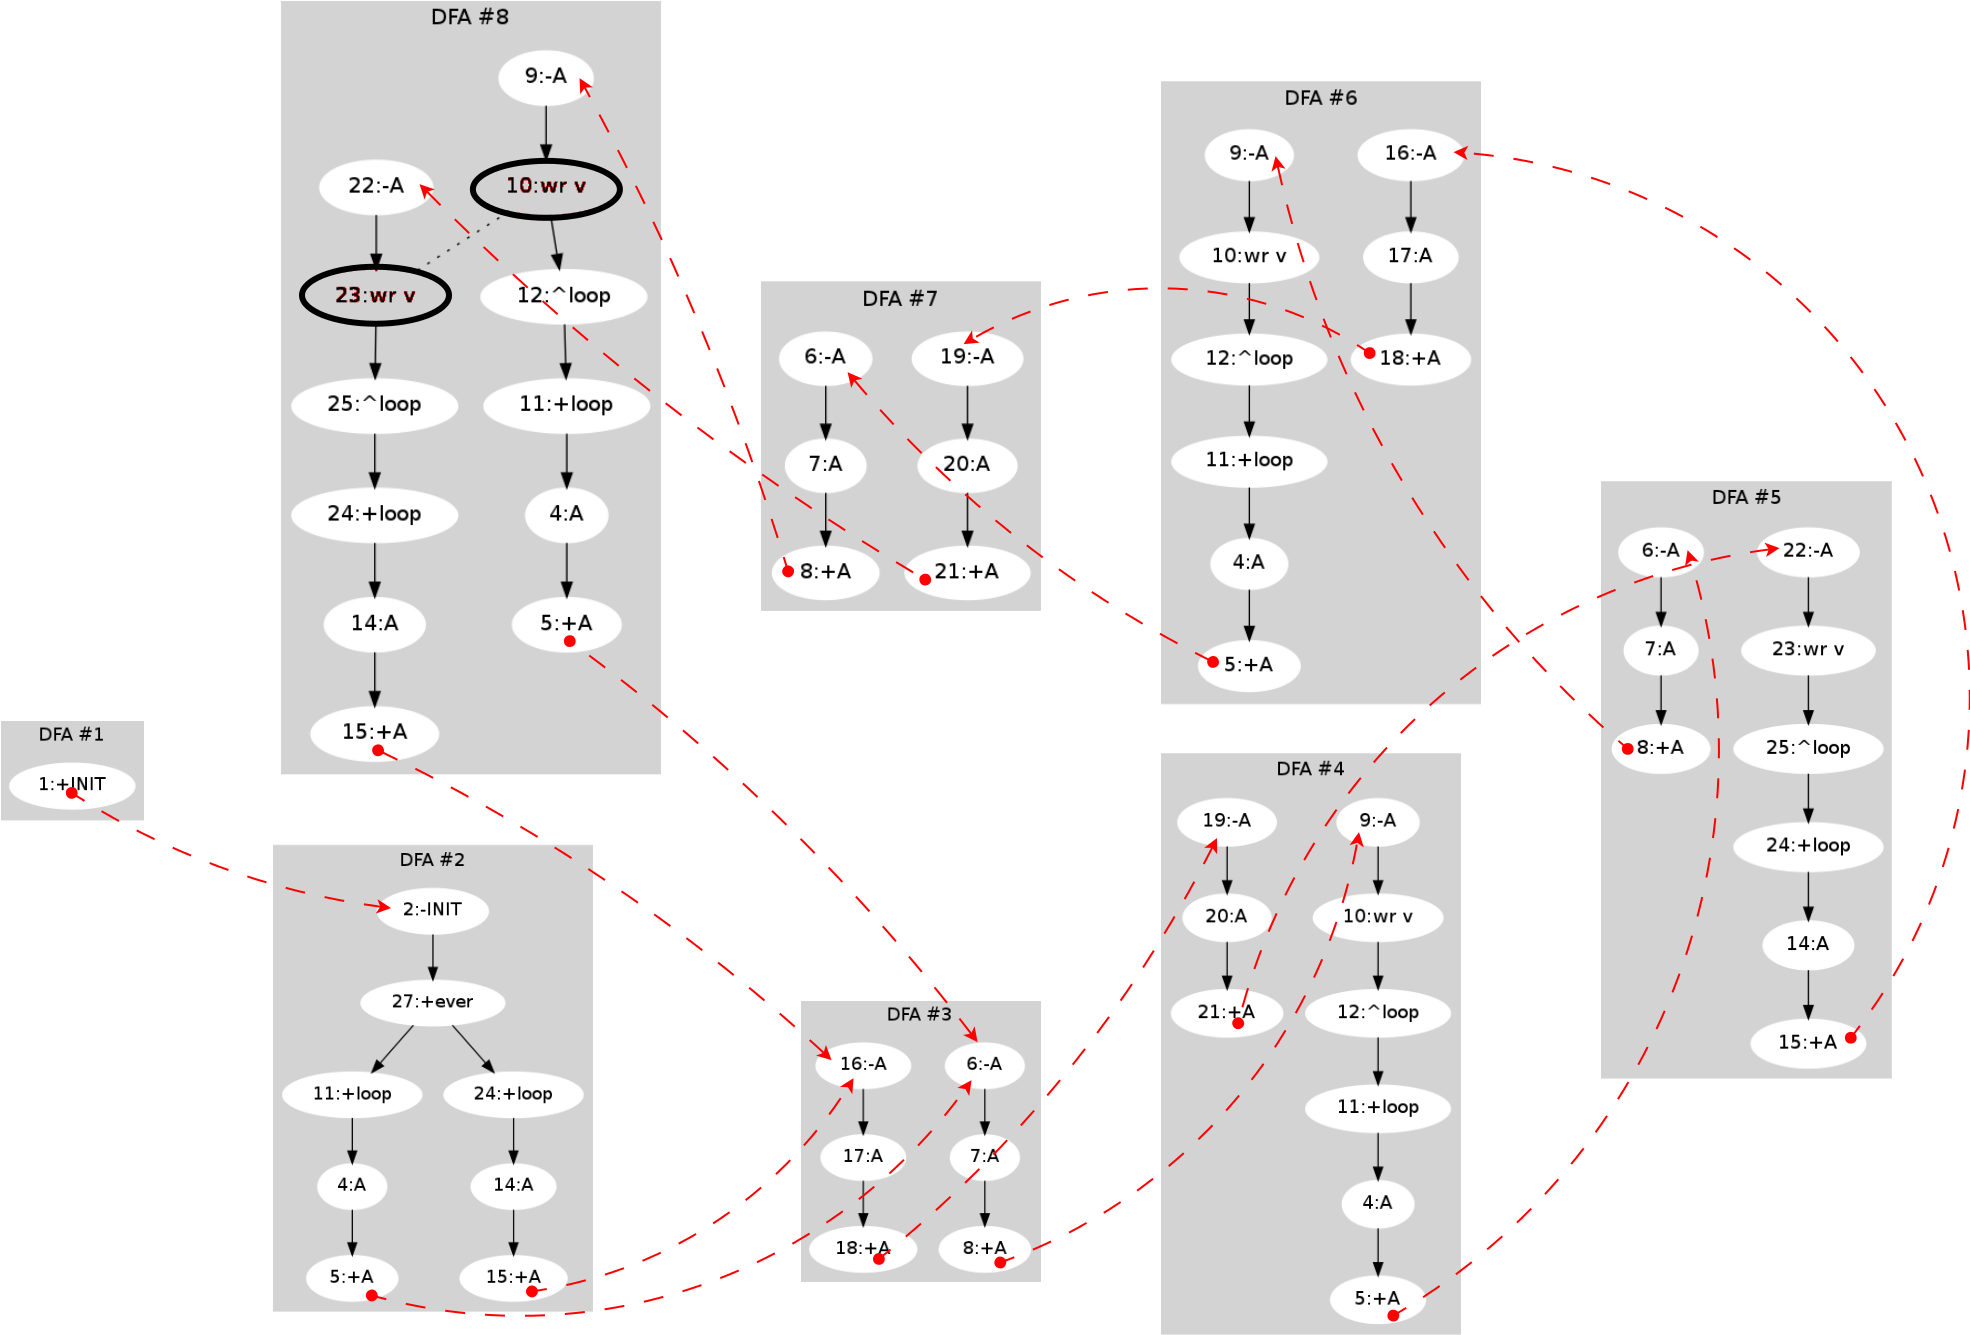
\includegraphics[scale=0.25]{dfa/dfa.png}
\caption{ DFA for the nondeterministic example.
\label{fig:dfa}
}
\end{figure*}

Determinism is usually a desired safety property, making concurrent programs 
predictable and easier to debug.

Concurrency in \CEU{} is characterized when two or more trails segments execute 
during the same reaction chain.
For instance, in the following example, the assignments run concurrently:
{\small
\begin{verbatim}
        int v;
        par/and do
            v = 1;
        with
            v = 2;
        end
\end{verbatim}
}
while in
{\small
\begin{verbatim}
        input void A, B;
        int v;
        par/and do
            await A;
            v = 1;
        with
            await B;
            v = 2;
        end
\end{verbatim}
}
there is no possible concurrency between the assignments, as $A$ and $B$ are 
external events and cannot happen at the same time (by \CEU's definition of 
time).

% TODO: prove
There are three possible sources of nondeterminism in \CEU:
\emph{concurrent access to variables},
\emph{concurrent access to internal events},
and \emph{concurrent $C$ calls}.

During compile time, \CEU{} performs a \emph{temporal analysis} in order to 
detect nondeterminism in programs.
The static analysis generates a deterministic finite automata that represents a 
program and covers exactly all possible points it can reach during runtime.
% TODO: claim

%\newpage
As an example, the DFA in Figure~\ref{fig:dfa} corresponds to the program in 
Figure~\ref{lst:ceu:det}.
In state \emph{DFA \#8} (after six occurrences of $A$) the variable \code{v} is 
accessed concurrently (note the outlined nodes), qualifying a nondeterministic 
behavior in the program, which is refused at compile time.

\begin{figure}[t]
\rule{8.5cm}{0.37pt}
{\small
\begin{verbatim}
    input void A;
    int v;
    par do
       loop do
          await A;
          await A;
          v = 1;
       end
    with
       loop do
          await A;
          await A;
          await A;
          v = 2;
       end
    end
\end{verbatim}
}
\caption{ A nondeterministic program.
\label{lst:ceu:det}
}
\end{figure}

% VARIABLES
% INTERNAL EVENTS

If a variable is written in a trail segment, it cannot be read or written in 
any other concurrent trail segment.
For internal events, the reasoning is similar: if an event is emitted, it 
cannot be awaited or emitted in any other concurrent trail segment.

% C CALLS

Regarding concurrent $C$ calls, \CEU{} supports annotations that allow specific 
functions to run concurrently with others.
Consider the following program:
{\small
\begin{verbatim}
    par/and do
       _led1On();
    with
       _led2On();
    end
\end{verbatim}
}
The two calls affect different leds, and the order each led is turned on cannot 
be perceived in practice.
Nonetheless, \CEU{} is strict about determinism and refuses this program by 
default.

The \code{pure} modifier of \CEU{} specifies functions that may run 
concurrently with any other function in the program, while the 
\code{deterministic} modifier specifies sets of functions that may run 
concurrently among them.

%\newpage
For instance, in the following code:
{\small
\begin{verbatim}
    pure _abs;
    deterministic _led1On,  _led2On;
    deterministic _led1Off, _led2Off;
\end{verbatim}
}
The function \code{\_abs} may run concurrently with any other functions, while 
\code{\_led1On/\_led2On} and \code{\_led1Off/\_led2Off} may run concurrently 
among them.

% WALL-CLOCK TIME

Finally, the temporal analysis of \CEU{} also embraces the semantics for 
wall-clock time.
The program
{\small
\begin{verbatim}
    int v;
    par/or do
        await 50ms;
        await 49ms;
        v = 1;
    with
        await 100ms;
        v = 2;
    end
\end{verbatim}
}
is deterministic, while the program
{\small
\begin{verbatim}
    int v;
    par/or do
        loop do
            await 10ms;
            v = 1;
        end
    with
        await 100ms;
        v = 2;
    end
\end{verbatim}
}
is nondeterministic, as the variable \code{v} is accessed concurrently every 
ten iterations of the first trail.

Note that \CEU{} may refuse some deterministic programs (the so called 
\emph{false positives}).
For instance, the following program is deterministic, but is recognized as 
nondeterministic by \CEU:
{\small
\begin{verbatim}
    int v;
    par/and do
        v = 1;
    with
        v = 1;
    end
    return v;
\end{verbatim}
}
Programs that access the same variables concurrently are always detected as 
nondeterministic, regardless of the values being assigned or read.

\subsection{Asynchronous execution}
\label{sec:ceu:async}

The main limitation of the synchronous execution model is its inability to 
perform long computations requiring unbounded loops.
\emph{Asynchronous blocks} fill this gap in \CEU{} and can contain unbounded 
loops that run asynchronously with the rest of the program (referred to as the 
\emph{synchronous side}).

\begin{figure}[t]
\rule{8.5cm}{0.37pt}
{\small
\begin{verbatim}
 1:  par/or do
 2:     int ret = async do
 3:        int num=10, fat=1;
 4:        loop do
 5:           if num == 0 then
 6:              return fat;
 7:           else
 8:              fat = fat * num;
 9:              num = num - 1;
10:           end
11:        end
12:     end;
13:     _printf("fat: %d\n", ret);
14:  with
15:     await 10ms;
16:  end
\end{verbatim}
}
\caption{ A program with a long computation.
\label{lst:ceu:async}
}
\end{figure}

The program in Figure~\ref{lst:ceu:async} returns the factorial of $10$.
The loop (lines 4-11) must be inside the \code{async} (lines 2-12) as it 
contains no await statements.
The \code{return} statement (line 6) terminates the asynchronous execution 
setting the variable \code{ret} (line 2).
We use a watchdog in the enclosing \code{par/or} to cancel the computation if 
it takes longer than $10$ms (line 15).

\CEU{} specifies that asynchronous code cannot execute when there are pending 
input events in the synchronous side, which always has higher priority.
It gives no warranty that an \code{async} will ever terminate.
Also, to preserve the disciplined synchronous semantics of \CEU{}, asynchronous 
blocks cannot use parallel blocks, cannot await input events, cannot manipulate 
internal events, and cannot assign to variables defined in outer blocks.

From the synchronous perspective, an \code{async} can be thought as an external 
process that generates an input event back into the program when it terminates.
The following code express this idea:

{\small
\begin{verbatim}
  _start_NNN();    // NNN is an unique identifier
  ret = await NNN; //   that represents the async
\end{verbatim}
}

The call to \code{\_start\_NNN()} requests the asynchronous computation to 
start, while the subsequent ``\code{await NNN}'' resumes when the computation 
terminates, yielding its final result.

This equivalence emphasizes that asynchronous blocks have a localized impact on 
the synchronous side of programs (to be discussed in 
Section~\ref{sec:ceu:gals}).

\subsection{Simulation in \CEU}
\label{sec:ceu:simul}

Simulation is an important aspect in cross-compiling platforms, such as 
embedded systems.
It is usually employed to test applications before deploying them on the target 
platform.
However, simulators are usually inaccurate, may require additional knowledge to 
operate, and vary among different developing platforms.

\CEU{} can simulate programs in the language itself, not depending on any 
external tool to test its programs: asynchronous blocks are allowed to emit 
input events and also events that represent the passage of wall-clock time 
towards the synchronous side of the program.
%Input events from asynchronous blocks go through the same queue for ``real'' 
%events---once in the input queue, there is no distinction among them.
This way, it is easy to simulate and test the execution of programs with total 
control and accuracy with regard to the order of input events---all is done 
with the same language and inside the programs themselves.

Note that in a reactive language, a program execution depends solely on the 
events it receives from the environment.
Also, in a deterministic program, the exact timings for the incoming events are 
irrelevant to the application outcome, only the order they arrive.

\begin{figure}[t]
\rule{8.5cm}{0.37pt}
{\small
\begin{verbatim}
 1:   input int Start;
 2:   int v = await Start;
 3:   par/or do
 4:      loop do
 5:         await 10min;
 6:         v = v + 1;
 7:      end
 8:   with
 9:      await 1h35min;
10:   end
\end{verbatim}
}
\caption{ The program to be simulated.
\label{lst:ceu:simul:1}
}
\end{figure}

\begin{figure}[t]
\rule{8.5cm}{0.37pt}
{\small
\begin{verbatim}
 0:   par/or do
(1-10):  // ORIGINAL CODE
11:      _assert(v == 19);
12:   with
13:      async do
14:         emit Start = 10;
15:         emit 1h35min;
16:      end
17:      _assert(0);
18:   end
\end{verbatim}
}
\caption{ A program that embeds code in Figure~\ref{lst:ceu:simul:1} and 
simulates it.
\label{lst:ceu:simul:2}
}
\end{figure}

Suppose we want to simulate the execution of the program in 
Figure~\ref{lst:ceu:simul:1}, which initially awaits the input event $Start$ 
and then increments $v$ every $10$ minutes during $1$ hour and $35$ minutes.
To test this code, we simulate the occurrence of the event $Start$ and the 
passage of \code{1h35min} in a parallel trail, as shown in 
Figure~\ref{lst:ceu:simul:2}.
The sequence of execution for the simulation will be as follows:

{\small
\begin{enumerate}
\setlength{\itemsep}{0pt}
\item The original code (lines 1-10) executes before the \code{async} and 
initially awaits the event \code{Start} (line 2).
\item The \code{async} (lines 13-17) begins, emits \code{Start=10} (line 14) 
and is suspended (the original code takes the priority again).
\item The original code resumes and awaits \code{10min} and \code{1h35min} in 
parallel trails (lines 5 and 9).
\item The \code{async} resumes and signals that \code{1h35min} have elapsed 
(line 15).
\item The original code completely reacts to all time: the loop iterates 
exactly $9$ times (lines 4-7) before the trail awaiting \code{1h35min} resumes 
(line 9) and terminates the innermost \code{par/or}.
The assertion test on line 11 executes before the one on line 17 (which never 
executes due to the outermost \code{par/or}) and terminates the program 
successfully.
\end{enumerate}
}

The original code remains unmodified and is simply pasted into the template 
that runs the simulation in parallel.
With the proper tools, this integration can be made even simpler (e.g. we 
developed a framework to run tests for the implementation of \CEU{} with 
hundreds of programs and test cases defined in separate).

It should be clear from the example that simulation does not test true I/O, 
only the program behavior given an arbitrary input sequence.
For instance, the simulation does not take $1$ hour to complete, but actually a 
negligible time.
Also, simulation can be employed---with the exact same behavior---in the 
developing platform (given \CEU{} is available) or in the target platform.

\subsection{GALS execution}
\label{sec:ceu:gals}

\CEU{} complies with the GALS (\emph{globally asynchronous, locally 
synchronous}) model of computation, which states that local activities run 
synchronized with a common clock, while global activities run with independent 
clocks.
The \emph{globally asynchronous} part of \CEU{} is restricted to external input 
events, $C$ code, and asynchronous blocks, while the \emph{locally synchronous} 
part of \CEU{} extends to all other primitives, such as parallel compositions, 
variable manipulation, and internal events.

The temporal analysis of \CEU{} discussed in Section~\ref{sec:ceu:det} ensures 
that only the locally synchronous part of programs is deterministic.
Therefore, \CEU{} is not an absolutely deterministic language, that is, the 
behavior of programs may vary from execution to execution.

However, nondeterminism in \CEU{} is exclusively a consequence of globally 
asynchronous execution.
For instance, the program in Figure~\ref{lst:ceu:gals} is nondeterministic, 
given that the \code{async} runs for an undetermined time, and may terminate 
before or after the statement \code{await~1s}.
Even so, the \CEU{} compiler does not complain about nondeterminism, because 
the assignments cannot run concurrently.

\begin{figure}[t]
\rule{8.5cm}{0.37pt}
{\small
\begin{verbatim}
    int ret;
    par/or do
        async do
            ...     // a long computation
        end
        ret = 1;
    with
        await 1s;
        ret = 2;
    end
    return ret;
\end{verbatim}
}
\caption{ The assignments never run concurrently.
\label{lst:ceu:gals}
}
\end{figure}

Note that for simulation purposes, the asynchronous execution can be entirely 
guided by synchronous code, making programs fully deterministic.
For instance, the simulation example of Figure~\ref{lst:ceu:simul:2} can be 
repeated many times, with the exact same behavior.

\section{Demo applications}
\label{sec:demos}

To demonstrate the expressiveness of \CEU{}, we implemented three applications 
in different domains and platforms.

The first example explores Wireless Sensor Networks (WSNs), which are networks 
composed of a large number of tiny devices (known as ``motes'') capable of 
sensing the environment and communicating among them.
We integrated \CEU{} with the \emph{TinyOS} operating system~\cite{wsn.tos} in 
order to use the abstracted radio services the operating system provides for 
motes.

The second example uses the Arduino platform, a popular choice among hobbyists 
aiming to experiment with electronic components and software.
Here, we cannot rely on device drivers and abstract services, as the I/O 
devices and pin connections vary from application to application.
In this context, we make extensive use of thin libraries for specific devices 
and program directly in the ``bare metal''.

The third example uses \CEU{} with the SDL graphics library%
\footnote{\url{http://www.libsdl.org}} under linux.
With a more powerful platform, we can explore some simulation techniques that 
require fast processing.

The three demos also illustrate different ways to integrate \CEU{} with an 
underlying platform.

For TinyOS, we developed a binding that maps all OS services to \CEU.
As TinyOS is event-driven, we intercept every possible event it can generate 
and emit a corresponding external input event in \CEU.
The binding is generic and applications can be developed entirely in \CEU.

For Arduino, we do not know in advance which I/O devices are available, hence, 
it is impossible to provide a unique high-level binding.
Instead, we developed a binding that generates events that notify changes on 
pins used as input ports in the \CEU{} program.

For SDL, we opted to use the ``standalone'' binding of \CEU{}, which starts the 
application and expects it to generate all input events to itself (inside 
asynchronous blocks).

The applications are somewhat simple to fit the paper (ranging from 70 to 200 
lines), but still complete enough to explore the programming techniques 
promoted by \CEU{}.

\subsection{WSN ring}
\label{sec:demos:ring}

In the first demo, we implement a fixed ring topology with three motes placed 
side by side within their radio ranges.%
\footnote{The complete source code and a video demo for the ring application 
can be found at \url{http://www.ceu-lang.org/onward/\#ring}.}

All motes should follow the same behavior: receive a message with an integer 
counter, show it on the leds, wait for $1$ second, increment the counter, and 
forward it to the mote on its right.
Note that using fixed topologies and running the same application in all motes 
are common practices in the context of WSNs.

As the topology constitutes a ring, the counter will be incremented forever 
while traversing the three motes.
If a mote does not receive a message within $5$ seconds, it should blink the 
red led every $500$ milliseconds until a new message is received.
%This behavior requires that both network-down/up events are handled.
In a ring topology, communications traverse all motes, and the network goes 
down with a failure in a single mote, making tests much easier.

The mote with \emph{id=0} is responsible for initiating the process at boot 
time, and also when the network is down.
On perceiving the failure, mote $0$ should wait for $10$ seconds before 
retrying the communication.

The code in Figure~\ref{lst:demos:ring:1} shows the communicating trail, which 
receives and forwards the messages forever.
The code is an endless loop that first awaits a radio message (line 2), gets a 
pointer to its data region (line 3), shows the received counter on the leds 
(line 4), and then awaits $1$s (line 5) before incrementing the counter in the 
message (line 6) and forwarding it to the next mote (line 7).

\begin{figure}[t]
\rule{8.5cm}{0.37pt}
{\small
\begin{verbatim}
 1:  loop do
 2:     _message_t* msg = await Radio_receive;
 3:     int* cnt = _Radio_getPayload(msg);
 4:     _Leds_set(*cnt);
 5:     await 1s;
 6:     *cnt = *cnt + 1;
 7:     _Radio_send((_TOS_NODE_ID+1)%3, msg);
 8:  end
\end{verbatim}
}
\caption{ Communicating trail for the ring application.
\label{lst:demos:ring:1}
}
\end{figure}

Because this code does not handle failures, it is straight to the point and 
easy to follow.
Actually, this is the final code for this task, as the task for handling errors 
is placed in a parallel trail.

Note that the program uses several services provided by the underlying 
operating system as $C$ functions (leds and radio facilities), and none of 
these calls are blocking.

To handle failures, we use a monitoring trail in parallel with the 
communicating trail, as Figure~\ref{lst:demos:ring:2} shows.
The network-down behavior constitutes the lines 12 to 24.
After $5$ seconds of inactivity is detected (line 12), two new activities run 
parallel: one that retries the communication every $10$ seconds (lines 14-17) 
by signaling the internal event \code{retry}; and another that blinks the red 
led every $500$ milliseconds (lines 19-23).

\begin{figure}[t]
\rule{8.5cm}{0.37pt}
{\small
\begin{verbatim}
 0:  par do
(1-8):  // COMMUNICATING TRAIL
 9:  with
10:     loop do
11:        par/or do
12:           await 5s;
13:           par do
14:              loop do
15:                 emit retry;
16:                 await 10s;
17:              end
18:           with
19:              _Leds_set(0);
20:              loop do
21:                 _Leds_led0Toggle();
22:                 await 500ms;
23:              end
24:           end
25:        with
26:           await Radio_receive;
27:        end
28:     end
29:  end
\end{verbatim}
}
\caption{ Monitoring trail for the ring application.
\label{lst:demos:ring:2}
}
\end{figure}

The trick to restore the normal behavior of the network is to await the 
\code{Radio\_receive} event (line 26) in a \code{par/or} (line 11) with the 
network-down behavior to kill it whenever the network link is restored.
By surrounding everything with a \code{loop} (line 10), we ensure that the 
error detection is continuous.

Note that both the communicating trail and the monitoring trail waits for the 
event \code{Radio\_receive} (lines 2 and 26, respectively), and both react 
concurrently to it.
The first is responsible for handling the message and forwarding it, while the 
second just kills the network-down behavior (the blinking red led).

Finally, we need to code the initiating/retrying process that sends the first 
message from the mote with \emph{id=0}.
As expected we place the code in parallel with the other activities, as 
Figure~\ref{lst:demos:ring:3} shows.

\begin{figure}[t]
\rule{8.5cm}{0.37pt}
{\small
\begin{verbatim}
 0:  par do
(1-8):   // COMMUNICATING TRAIL (lines 1-8)
 9:  with
(10-28): // MONITORING TRAIL (lines 10-28)
29:  with
30:     if _TOS_NODE_ID == 0 then
31:        loop do
32:           _message_t msg;
33:           int* cnt = _Radio_getPayload(&msg);
34:           *cnt = 1;
35:           _Radio_send(1, &msg)
36:           await retry;
37:        end
38:     else
39:        await forever;
40:     end
41:  end
\end{verbatim}
}
\caption{ Retrying trail for the ring application.
\label{lst:demos:ring:3}
}
\end{figure}

We start by checking if the mote has \emph{id=0} (line 30).
If this is not the case, we simply await forever%
\footnote{\code{forever} is a reserved keyword in \CEU, and represents an 
external input event that never occurs.}
on this trail (line 39).
Otherwise, the \code{loop} (lines 31-37) sends the first message as soon as the 
mote is turned on (line 35).
It then waits for a \code{retry} emit (line 36) to loop and resend the initial 
message.

The example shows how complementary activities in an application can be written 
in separate and need not to be mixed in the code.
The activities are then combined together through parallel compositions and 
communication via internal events to achieve the intended behavior.

The complete source code is less than 70 lines and includes all definitions and 
code to initialize the radio.

As a final consideration, we can extend the idea of compositions to a new level 
by combining different \emph{applications} together.
In the context of WSNs, it is usually difficult to physically recover motes in 
a deployed network, and by combining multiple applications in a single image, 
we can switch their execution remotely via radio.

The program in Figure~\ref{lst:demos:ring:4} illustrates this idea.
The input event \code{Switch} (line 1) is used to request application switches 
remotely.%
\footnote{ We are assuming the existence of an hypothetical high-level event 
\code{Switch} that abstracts the radio protocol for requests to change the 
current running application. }
Initially, the code behaves as application $1$ (lines 7-9), but is also waiting 
for a \code{Switch} request in parallel (line 5).
Whenever a new request occurs, the \code{par/or} terminates, kills the running 
application, and restarts as the requested application.
The \code{await forever} statement (line 13) ensures that a terminating 
application does not restart by itself.

\begin{figure}[t]
\rule{8.5cm}{0.37pt}
{\small
\begin{verbatim}
 1:   input int Switch;
 2:   int cur_app = 1;
 3:   loop do
 4:      par/or do
 5:         cur_app = await Switch;
 6:      with
 7:         if cur_app == 1 then
 8:            // CODE for APP1
 9:         end
10:         if cur_app == 2 then
11:            // CODE for APP2
12:         end
13:         await forever;
14:      end
15:   end
\end{verbatim}
}
\caption{ Composition of two applications.
\label{lst:demos:ring:4}
}
\end{figure}

This idea can also be used to \emph{reboot} a mote remotely, in the case of a 
strange behavior in an application.

Note that the final ROM image on the mote requires the sum of all installed 
applications.
However, as the applications never execute in parallel, the requirement for RAM 
is equal to the highest footprint among all installed applications (to be 
discussed in Section~\ref{sec:impl:memory}).

\subsection{Arduino ship game}

In this demo, we control a ship that moves on space and has to avoid collisions 
with meteors until reaching a finish line.%
\footnote{The complete source code and a video demo for the ship application 
can be found at \url{http://www.ceu-lang.org/onward/\#ship}.}

We use an Arduino connected to a two-row LCD display and two buttons that 
control the ship.
Figure~\ref{fig:ship} shows the picture of a running quest.

\begin{figure}[t]
\centering
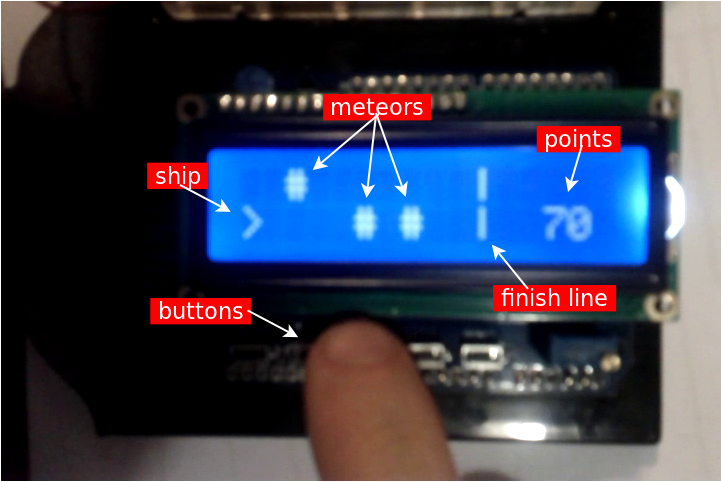
\includegraphics[scale=0.33]{ship.png}
\caption{ The ``ship'' game
\label{fig:ship}
}
\end{figure}

\begin{figure}[t]
\rule{8.5cm}{0.37pt}
{\small
\begin{verbatim}
 1:  loop do
(2-12): // CODE 1: set game attributes
13:
14:     _map_generate();
15:     _redraw(step, ship, points);
16:     await Key;  // starting key
17:
18:     win =
(19-45): // CODE 2: the central loop
46:
(47-60): // CODE 3: game over
61:  end
\end{verbatim}
}
\caption{ The outermost loop for the ship game.
\label{lst:demos:ship:1}
}
\end{figure}

We specify the behavior of the game along with the code and follow a top-down 
approach.
The outermost loop of the game in Figure~\ref{lst:demos:ship:1} is responsible 
for restarting the game every new phase or on ``game over''.
The complete code is constituted of \code{CODE~1}, \code{CODE~2}, and 
\code{CODE~3}, which are expanded further.

Every time the loop is executed, it resets the game attributes, such as points 
and speed (\code{CODE 1}, lines 2-12), generates a new map and redraws it on 
screen (lines 14-15).
Then, it waits for a starting key (line 16), and executes the main logic of the 
game in the central loop (\code{CODE 2}, lines 18-45) until the ship reaches 
the finish line or collides with a meteor.
Based on the return status (line 18), the ``game over'' code (\code{CODE 3}, 
lines 47-60) may display an animation before restarting the game.

The game attributes (\code{CODE 1}, in Figure~\ref{lst:demos:ship:2}) change 
depending on the result of the previous iteration of the outermost loop.

\begin{figure}[t]
\rule{8.5cm}{0.37pt}
{\small
\begin{verbatim}
     // CODE 1: set game attributes
 2:  ship = 0;          // 1st LCD row
 3:  if !win then
 4:     dt     = 500;   // game speed (500ms/step)
 5:     step   = 0;     // current step
 6:     points = 0;     // number of steps alive
 7:  else
 8:     step = 0;
 9:     if dt > 100 then
10:        dt = dt - 50;
11:     end
12:  end
\end{verbatim}
}
\caption{ The attributes settings for the ship game.
\label{lst:demos:ship:2}
}
\end{figure}

For the first game execution and whenever the ship collides with a meteor, 
variable \code{win} is set to 0%
\footnote{We omitted all global declarations in the code.},
hence, the attributes are reset to their initial values (lines 4-6).
Otherwise, if the player reached the finish line (\code{win=1}), then the game 
gets faster, keeping the current points (lines 8-11).

The central loop of the game (\code{CODE 2}, in Figure~\ref{lst:demos:ship:3}) 
is responsible for moving the ship as time elapses and for checking whether the 
ship reached the finish line or collided with a meteor.

\begin{figure}[t]
\rule{8.5cm}{0.37pt}
{\small
\begin{verbatim}
     // CODE 2: the central loop
19:  par do
20:     loop do
21:        await(dt*1000);
22:        step = step + 1;
23:        _redraw(step, ship, points);
24:
25:        if _MAP[ship][step] == '#' then
26:           return 0;  // a collision
27:        end
28:
29:        if step == _FINISH then
30:           return 1;  // finish line
31:        end
32:
33:        points = points + 1;
34:     end
35:  with
36:     loop do
37:        int key = await Key;
38:        if key == _KEY_UP then
39:           ship = 0;
40:        end
41:        if key == _KEY_DOWN then
42:           ship = 1;
43:        end
44:     end
45:  end;
\end{verbatim}
}
\caption{ The central loop for the ship game.
\label{lst:demos:ship:3}
}
\end{figure}

The central loop is actually split in two loops in parallel, one to run the 
game steps (lines 20-34), and the other to handle input from the player (lines 
36-44).

The game steps run periodically, depending on the current speed of the game 
(line 21).
For each loop iteration, the step is incremented and the screen is redrawn 
(lines 22-23).
Then, the ship is checked for collision with meteors (lines 25-27), and with 
the finish line (lines 29-31).
\CEU{} supports returning from blocks with an assignment, hence, lines 26 and 
30 escape the whole \code{par} and assign to the \code{win} variable in the 
outer loop (line 18).
The points are incremented before each iteration of the loop (line 33).

To handle input events, we wait for key presses in a loop (line 37) and change 
the ship position accordingly (lines 39, 42).
Note that there are no possible race conditions on variable \code{ship} because 
the two loops in the \code{par} statement react to different events (i.e. 
wall-clock time and keys).

After returning from the central loop, we run the code for the ``game over'' 
behavior, in Figure~\ref{lst:demos:ship:4}, which starts an animation if the 
ship collided with a meteor.

\begin{figure}[t]
\rule{8.5cm}{0.37pt}
{\small
\begin{verbatim}
     // CODE 3: game over
47:  par/or do
48:     await Key;
49:  with
50:     if !win then
51:        loop do
52:           await 100ms;
53:           _lcd.setCursor(0, ship);
54:           _lcd.write('<');
55:           await 100ms;
56:           _lcd.setCursor(0, ship);
57:           _lcd.write('>');
58:        end
59:     end
60:  end
\end{verbatim}
}
\caption{ The ``game over'' code for the ship game.
\label{lst:demos:ship:4}
}
\end{figure}

The animation loop (lines 51-58) continuously displays the ship in the two 
directions, suggesting that it has hit a meteor.
The animation is interrupted when the player presses a key (line 48), 
proceeding to the game restart.

Finally, we need to generate the key events from the program itself, as we use 
a third-party push-button component not present in all Arduino boards.
For this, we place the whole program in parallel with the input event 
generator, as Figure~\ref{lst:demos:ship:5} shows.

\begin{figure}[t]
\rule{8.5cm}{0.37pt}
{\small
\begin{verbatim}
 0:  par do
(1-61): // CODE FOR THE GAME
62:  with
63:     int key = _KEY_NONE;
64:     loop do
65:        int read1 = _analog2key(_analogRead(0));
66:        await 50ms;
67:        int read2 = _analog2key(_analogRead(0));
68:        if read1==read2 && key!=read1 then
69:           key = read1;
70:           if key != _KEY_NONE then
71:              async do
72:                 emit Key = read1;
73:              end
74:           end
75:        end
76:     end
77:  end
\end{verbatim}
}
\caption{ Event generator for the ship game.
\label{lst:demos:ship:5}
}
\end{figure}

The code samples data of an analog port with a delay of $50$ms to avoid 
bouncing (lines 65-67).
If two consecutive reads point to the same key and they are different from the 
previous change (line 68), then we change the key (line 69) and generate a new 
event (in the case of a key press, lines 70-74).
The \code{async} block is mandatory for generating input events to the program.

The static analysis complains about concurrent $C$ calls of the game code (i.e.  
\code{\_map\_generate} and \code{\_redraw}) against the event generator code 
(i.e. \code{\_analog2key} and \code{\_analogRead}).
By annotating functions with proper modifiers, we get rid of all 
nondeterministic errors:

{\small
\begin{verbatim}
    pure _analog2key;   // just a mapping function
    deterministic _analogRead, _map_generate;
    deterministic _analogRead, _redraw;
\end{verbatim}
}

The complete source code is around 170 lines and also contains $C$ definitions 
to generate the map, redraw the scene on the LCD, etc.

\subsection{SDL game simulation}

In the third demo, we implement a simple game to experiment with simulation 
techniques.
Our goal is to show how a self-contained application can be embedded 
\emph{unmodified} in an enclosing environment that may re-execute the 
application in many ways with the same behavior.
%\footnote{The motivation behind this demo came from a recent talk by Bret 
%Victor:
%}

In our game%
\footnote{The complete source code and a video demos for the Mario Bros 
applications can be found at \url{http://www.ceu-lang.org/onward/\#mario}.}, 
Mario Bros moves in one direction with a constant speed and jumps in reaction 
to key presses.
A turtle moves in the opposite direction randomly.
In the case of a collision with the turtle, Mario is thrown back forcedly.
The game is intentionally simple as our main objective is to play with 
simulation.
Figure~\ref{lst:demos:mario:1} shows the code for the game.

\begin{figure}[!]
\rule{8.5cm}{0.37pt}
{\small
\begin{verbatim}
 1:  input    int  Seed;
 2:  input    void Key;
 3:  input    void Step;
 4:  internal void collision;
 5:
 6:  int seed = await Seed;
 7:  _srand(seed);
 8:
 9:  int mario_x  = 10;
10:  int mario_dx = 1;
11:  int mario_y  = 236;
12:  int mario_dy = 0;
13:
14:  int turtle_x  = 600;
15:  int turtle_y  = 250;
16:  int turtle_dx = 0;
17:
18:  _redraw(mario_x,mario_y, turtle_x,turtle_y);
19:
20:  par do
21:      loop do
22:          await 50ms;
23:          turtle_dx = - (_rand()%4-1);
24:      end
25:  with
26:      loop do
27:          int v =
28:              par do
29:                  await Key;
30:                  return 1;
31:              with
32:                  await collision;
33:                  return 0;
34:              end;
35:          if v == 1 then
36:              mario_dy = -2;
37:              await 500ms;
38:              mario_dy = 2;
39:              await 500ms;
40:              mario_dy = 0;
41:          else
42:              mario_dx = -4;
43:              await 300ms;
44:              mario_dx = 1;
45:          end
46:      end
47:  with
48:      loop do
49:          await Step;
50:          mario_x  = mario_x  + mario_dx;
51:          mario_y  = mario_y  + mario_dy;
52:          turtle_x = turtle_x + turtle_dx;
53:          if !( mario_x+32<turtle_x ||
54:                turtle_x+32<mario_x ) then
55:              emit collision;
56:          end
57:          _redraw(mario_x,mario_y,
58:                  turtle_x,turtle_y);
59:      end
60:  end
\end{verbatim}
}
\caption{ Code for the Mario Bros
\label{lst:demos:mario:1}
}
\end{figure}

%TODO: figure

%\newpage
The first three lines specify the game input interface.
\code{Seed} is an input event that is emitted once to be used in the generation 
of random numbers.
\code{Key} is emitted whenever the player presses a key to jump.
\code{Step} is emitted every $10$ms and conducts the execution of the game in 
discrete steps.
The internal event \code{collision} (line 4) is generated whenever Mario 
collides with the turtle.

The game starts waiting for the event \code{Seed} (line 6), which is expected 
to be generated by the environment at the beginning of the game.
Then, it proceeds to set the initial positions and speeds for the characters.
Mario starts on the left side of the screen and initially moves at a constant 
speed to the right (lines 9-12).
The turtle starts on the right side and initially does not move (lines 14-16).
The characters are then displayed on the screen (line 18).

The actual game action follows with three loops that run in parallel (lines 
20-60).

The first loop (lines 21-24) randomly changes the turtle speed every $50$ms.

The second loop (lines 26-46) is responsible for controlling the speed of 
Mario, which can be either reacting to a key press (line 29) or to a collision 
with the turtle (line 32).
Whatever happens first is assigned to variable \code{v} (line 27), and the 
speed of Mario in one of the axis is changed temporarily (lines 35-45).
During this period, new key presses and collisions are ignored.

The third loop (lines 48-59) reacts to event \code{Step} and is responsible for 
updating the characters positions (lines 50-52), checking for collisions (lines 
53-56), and redrawing the screen (line 57-58).

We embed the presented game code in three different environments.
The first variation just provides input for the game (e.g. keys presses and 
wall-clock time) and does not interfere with it.
The second variation also shows the replay of the game after $10$ seconds of 
gameplay (in an increased speed).
The third variation shows the replay running backwards.

In the remainder of this section, we only discuss the third variation, which 
encompasses all difficulties found in the other variations.

In order to exhibit the replay of the gameplay, we need to record the input 
sequence performed by the player and then re-execute the game from scratch by 
repeating the same input sequence.
As discussed in Section~\ref{sec:ceu:simul}, the behavior of a program in 
\CEU{} depends solely on the input order: re-executing a program with the same 
input must yield the exact same behavior.

However, we want the replay to execute backwards after $10$ seconds of gameplay 
(or $1000$ execution steps).
For instance, the last scene in the normal execution must be the first one in 
the replay.
To address this requisite, we simulate the passage of all $1000$ steps without 
any delay and without any redrawing of intermediate scenes.
Then, we redraw the last scene of the simulation and repeat the whole process, 
now for one step less (e.g. $9999$).

A possible source of nondeterminism in the game are the calls to \code{\_srand} 
and \code{\_rand} (lines 7,23), however, they become deterministic when we 
repeat the seed used in the original execution.

Figure~\ref{lst:demos:mario:2}~and~\ref{lst:demos:mario:3} shows the complete 
code for the game simulation.
As we are not using a preexisting SDL binding for \CEU{}, we need to emit all 
events from an \code{async} placed in parallel with the game.

\begin{figure}[t]
\rule{8.5cm}{0.37pt}
{\small
\begin{verbatim}
 1:  input void Restart;
 2:  par do
 3:     loop do
 4:        par/or do
 5:           // CODE FOR THE GAME
 6:        with
 7:           await Restart;
 8:        end
 9:     end
10:  with
11:     async do
12:        // CODE FOR THE EVENT GENERATOR
13:        int seed = _time(0);
14:        emit Seed = seed;
15:
16:        int[10] keys;   // keys vector
17:        keys[0] = -1;   // no keys so far
18:        int idx = 0;    // next key index
19:
20:        int step = 0;
21:        loop do
22:           _SDL_Event event;
23:           if _SDL_PollEvent(&event) then
24:              if event.type == _SDL_KEYDOWN then
25:                 keys[idx] = step;
26:                 idx = idx + 1;
27:                 keys[idx] = -1;
28:                 emit Key;
29:              end
30:           else
31:              _SDL_Delay(10);
32:              step = step + 1;
33:              emit 10ms;
34:              emit Step;
35:              if step == 1000 then
36:                 break;
37:              end
38:           end
39:        end
40:
41-71:     // CODE FOR THE BACKWARDS REPLAY
72:     end
73:  end
\end{verbatim}
}
\caption{ Code for the Mario Bros simulation.
\label{lst:demos:mario:2}
}
\end{figure}

The game code (line 5) runs in parallel with the \code{async} responsible for 
generating events (lines 11-72).
Also, we need to be able to restart the game from any point, so we use the 
event \code{Restart} (line 1) as a watchdog running in parallel with the game 
code (lines 3-9).

\begin{figure}[t]
\rule{8.5cm}{0.37pt}
{\small
\begin{verbatim}
41:        // CODE FOR THE BACKWARDS REPLAY
42:        int step_ref = 1000;
43:        loop do
44:           _redraw_on(0);
45:           emit Restart;
46:           emit Seed = seed;
47:
48:           step = 0;
49:           idx  = 0;
50:           loop do
51:              if step == keys[idx] then
52:                 emit Key;
53:                 idx = idx + 1;
54:              else
55:                 step = step + 1;
56:                 emit 10ms;
57:                 emit Step;
58:                 if step == step_ref then
59:                    break;
60:                 end
61:              end
62:           end
63:           _redraw_on(1);
64:           _redraw(0,0,0,0);
65:
66:           _SDL_Delay(1);
67:           step_ref = step_ref - 1;
68:           if step_ref == 0 then
69:              break;
70:           end
71:        end
\end{verbatim}
}
\caption{ Code for the Mario Bros simulation (cont.).
\label{lst:demos:mario:3}
}
\end{figure}

The event generator starts emitting the random \code{Seed}, which is saved on 
variable \code{seed} to be reused in the replay (lines 13-14).

We use the vector \code{keys} to record all steps in which the player presses a 
key (lines 16-18).
Each index on the vector holds the step in which a key was pressed.
Then, every time the player presses a key, the current step is written on the 
vector (lines 25-27).
The variable \code{step} (line 20) keeps track of the current running 
\code{Step}.

The loop in lines 21-39, continuously polls for key events to emit to the game 
(lines 22-29), and also emits wall-clock time and the event \code{Step} 
periodically (lines 30-38).
After $1000$ steps (i.e. $10$ seconds), we escape the event generator (lines 
35-37) and proceed to the replay code (lines 41-71).

With the original execution recorded, we can now re-execute the game by feeding 
it with the same input sequence as many times as desired, as 
Figure~\ref{lst:demos:mario:3} shows.

The variable \code{step\_ref} (line 42) varies from $1000$ to $0$ and guides 
the backwards simulation in the outermost loop following it (lines 43-71).
For each \code{step\_ref}, we first call \code{\_redraw\_on(0)} (line 44) to 
disable redrawing of intermediates scenes.
Then, we emit a \code{Restart} and the original \code{Seed} to the game (lines 
45-46) and simulate the execution in the innermost loop up to the current 
\code{step\_ref} (lines 50-62).
The innermost loop emits a \code{Key} event for each step matching the recorded 
vector (lines 51-53).
Also, it simulates the steps (lines 55-57), escaping the loop when reaching the 
current \code{step\_ref}.
After that, the simulation reached the last scene for the current 
\code{step\_ref}, so we redraw it on the screen (lines 63-64).
Before proceeding to the next outermost loop iteration (i.e. the previous 
step), we delay the execution to make the replay visible (lines 66-70).

Note that all variables in the code for the game are local to it, hence, they 
are reinitialized correctly after each \code{Restart}.
It is fundamental that all side effects in the game code are localized and do 
not extrapolate it.

In our example, the only exception to this rule is the call to \code{\_redraw}, 
which is handled with the specific tweak that enables and disables screen 
redrawing.

\section{Implementation of \CEU}
\label{sec:impl}

As a static language, much of the complexity of the implementation of \CEU{} 
resides in the compile phase.
Nonetheless, some complexity is left to the runtime phase, which has to handle 
multiple queues for active trails, asynchronous code, and wall-clock time.

The \CEU{} parser is written in \emph{LPeg}~\cite{lua.lpeg}, and converts a 
program into an \emph{abstract syntax tree (AST)} to be used in the following 
phases.

The program in Figure~\ref{lst:impl} is used as our guiding example for this 
section.

\begin{figure}[t]
\rule{8.5cm}{0.37pt}
{\small
\begin{verbatim}
    input int A, B, C;
    int ret;
    loop do
       par/or do
          int a = await A; // 1st trail
          int b = await B;
          ret = a + b;
          break;
       with
          par/and do       // 2nd trail
             await C;
          with
             await A;
          end
       end
    end
    ...                    // code after the loop
\end{verbatim}
}
\caption{ Guiding example for Section~\ref{sec:impl}.
\label{lst:impl}
}
\end{figure}

\subsection{Temporal analysis}

The \emph{temporal analysis} phase detects inconsistencies in \CEU{} programs, 
such as tight loops and the forms of nondeterminism, as discussed in Sections 
\ref{sec:ceu:bounded} and \ref{sec:ceu:det}.
It is also responsible for setting the priorities for trails (see further) and 
determining the sizes of the queues that are used during runtime.

The program AST is first converted into a graph that represents the execution 
flow.
Figure~\ref{fig:nfa} shows the corresponding graph for our example.

\begin{figure}[ht]
\centering
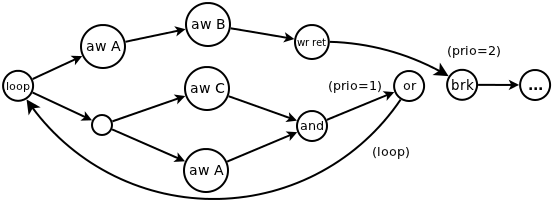
\includegraphics[scale=0.40]{nfa.png}
\caption{ Flow graph for our guiding example
\label{fig:nfa}
}
\end{figure}

By default, all nodes in a flow graph have priority $0$ (highest).
However, as the figure shows, nodes that represent the termination of 
\emph{par/ors} and loops have lower priorities (the outer, the lower).
The priority scheme is needed to avoid glitches during runtime, and is 
equivalent to traversing a dependency graph in topological order, as employed 
in functional reactive programming implementations.~\cite{frtime.embedding}

The flow graph is then converted to a DFA, as exemplified in 
Section~\ref{sec:ceu:det}.

\begin{comment}
From its starting node, the flow graph is traversed until reaching await 
nodes---every visited node is inserted into a new DFA state.
Then, every set of awaiting nodes for a given external event starts another DFA 
state.
\end{comment}

\subsection{Memory layout}
\label{sec:impl:memory}

\CEU{} favors a fine-grained use of trails, being common to use trails that 
await a single event.
For this reason, \CEU{} does not allocate per-trail stacks; instead, all data 
resides in fixed memory slots---this is true for the program variables as well 
as for temporary values and flags needed during runtime.
For instance, the first trail in the guiding example requires temporary slots 
to hold the locals \code{a} and \code{b}, while the second trail must keep 
flags to remember which sides of the \code{par/and} have already terminated.

Memory for trails in parallel must coexist, while statements in sequence can 
reuse it.
In the example, the code following the loop (identified as \code{...}) reuses 
all memory from the loop.

\CEU{} statically allocates a one dimension vector to hold all memory slots, 
whose size is the maximum the program uses at a given time.
A given position in the vector may hold different data (with variable sizes) 
during runtime.

\subsection{Gate allocation}
\label{sec:impl:gates}

Each await statement has an associated \emph{gate} that indicates whether it is 
currently active (awaiting) or not.
Gates for the same event are grouped in a list that is traversed whenever the 
event occurs, awaking the statements whose gates are active.
In contrast with memory slots, gates are global and cannot be reused in 
different parts of the program.

In the example, there is one gate for each of the four await statements.
For instance, when the event \code{A} occurs, its list of two gates is 
traversed in order to awake its currently active awaiting trails.

All gates are set to inactive when a program starts.
Once an await statement is reached, its corresponding gate is turned on.
Once an await statement awakes, its corresponding gate is turned off.

In \CEU, there is a strict relation between gates and trails.
A trail can be seen as a sequence of atomic operations with await statements
separating them.
If a trail is active, it must be awaiting an event.
Therefore, a trail can be destroyed by blindly setting all of its gates to 
inactive.
Also, gates in parallel trails use consecutive memory slots, hence, destroying 
trails in parallel is as easy as setting the respective range of gate slots to 
zero with a \code{memset} operation.
This is exactly what \CEU{} does to sibling trails when a \code{par/or} or 
\code{loop} terminates.

\begin{figure}[t]
\rule{8.5cm}{0.37pt}
{\small
\begin{verbatim}
   Sub_1:
      GATES[A1] = Aft_A;   // activates gate A1
      halt;                // awaits A
   Aft_A:
      GATES[A1] = 0;       // deactivates gate A1
      DATA[a]   = DATA[A]; // a = A
      GATES[B1] = Aft_B;   // activates gate B1
      halt;                // await B
   Aft_B:
      GATES[B1] = 0;       // deactivates gate B1
      DATA[b]   = DATA[B]; // b = B
      DATA[ret] = DATA[a]+DATA[b]; // ret = a+b
      halt;
\end{verbatim}
}
\caption{ Pseudo-code for a sequence of awaits.
\label{lst:impl:code:1}
}
\end{figure}

\subsection{Code generation}
\label{sec:impl:code}

The final output of the \CEU{} compiler is code in pure $C$, which is not only 
highly portable across platforms, but also omnipresent in embedded systems.
For some \CEU{} statements, such as calls and expressions, the conversion is 
straightforward and maps directly to $C$.

The biggest semantic mismatch between $C$ and \CEU{} resides in the await and 
parallel statements, which have no analogous in $C$.
Consider the follows sequence from the example:
{\small
\begin{verbatim}
    int a = await A;
    int b = await B;
    ret = a + b;
\end{verbatim}
}
It is clear that before performing the assignment to \code{ret}, the program 
must yield control to the environment twice to await the input events \code{A} 
and \code{B}.
Hence, the generated code must be split in three parts: before awaiting 
\code{A}, before awaiting \code{B}, and finally performing the addition and 
assignment.
Figure~\ref{lst:impl:code:1} shows the pseudo-code generated for that sequence.
  
Labels \code{Sub\_1}, \code{Aft\_A}, and \code{Aft\_B} represent entry points 
into the code, known as \emph{tracks}, held in gates and which \CEU{} spawns 
according to the occurring input event and state of gates.
Recall that locals such as \code{a} and \code{b} cannot be held on the stack, 
as the \code{halt} instruction yields control back to the environment between 
awaits.  

\CEU{} holds spawned tracks in a queue that is traversed respecting their 
priorities.
This way, a parallel statement simply inserts its tracks (one for each 
sub-block) into this queue and halts, letting the scheduler decide when they 
execute.

For instance, the \code{par/or} in the example spawns the track \code{Sub\_1} 
of the previous chunk:
{\small
\begin{verbatim}
    Par_1:
       enqueue Sub_1;
       enqueue Sub_2;
       halt;
    Sub_1:
        ...
    Sub_2:
        ...
    ...
\end{verbatim}
}
In the final code, illustrated in Figure~\ref{lst:impl:code:2}, the track 
labels become $C$ switch case labels, which are all enclosed by a loop that 
traverses the queue of spawned tracks (\code{Q\_TRACKS}).

\begin{figure}[t]
\rule{8.5cm}{0.37pt}
{\small
\begin{verbatim}
    while ( track = remove(Q_TRACKS) )
    {
    _SWITCH:
       switch (track) {
          case Par_1:
             enqueue Sub_1;
             enqueue Sub_2;
             break;             // halts
          case Sub_1:
             GATES[A1] = Aft_A; // activates gate A1
             break;             // awaits A
          case Sub_2:
             ...
          ...
       }
    }
\end{verbatim}
}
\caption{ Traversal of the queue for tracks.
\label{lst:impl:code:2}
}
\end{figure}

Note the \code{\_SWITCH} goto label, which is used for control-flow statements 
(i.e. loops and conditionals): in our example, the track \code{Aft\_B} must escape 
the loop after the assignment.
Its actual code is as follows:
{\small
\begin{verbatim}
   Aft_B:
      GATES[B1] = 0;       // deactivates gate B1
      DATA[b]  = DATA[B];  // b = B
      DATA[ret] = DATA[a]+DATA[b]; // ret = a+b
      track = Loop1_esc;   // escapes the loop
      goto _SWITCH;
\end{verbatim}
}

As the code suggests, all tracks execute atomically.
This way, even if the temporal analysis is turned off, there are no possible 
race conditions on shared variables.
A possible \CEU{} implementation exploring parallelism must ensure atomicity 
among tracks sharing state.

\subsection{Reactive execution}

As a reactive language, the execution of a program in \CEU{} is guided by the 
occurrence of external events.
From the implementation perspective, there are four external sources of input 
into programs, which are all exposed as functions in a $C$ API:

\begin{description}
\item[{\textbf\code{ceu\_go\_init}}:] initializes internal state (e.g. queues 
and gates) and executes the ``boot'' reaction.

\item[{\textbf\code{ceu\_go\_event}}:] executes the reaction for the received 
input id and associated data.

\item[{\textbf\code{ceu\_go\_time}}:] receives the current wall-clock time and 
checks for timeouts (running a reaction if needed).

\item[{\textbf\code{ceu\_go\_async}}:] executes a single loop iteration for the
next \code{async}, switching among them in a \emph{round robin} policy.
\end{description}

The functions take a bounded time to execute and represent a reaction chain in 
\CEU{}.
They also return a status code that says if the \CEU{} program has terminated 
after reacting to it.
Further calls to the API have no effect on terminated programs.

Note that \CEU{} code running from a call to \code{ceu\_go\_async} may emit an 
input event or the passage of time.
In this case, the $C$ implementation makes a tail call to the corresponding 
handler (i.e.  \code{ceu\_go\_event} or \code{ceu\_go\_time}), as synchronous 
code has higher priority.

The API reflects the \emph{global asynchronous} part of \CEU{}, as discussed in 
Section~\ref{sec:ceu:gals}.
A simple and opaque API hides local state from the environment, suggesting that 
the execution varies entirely according to the sequence (and parameters) of API 
calls.

The bindings for the specific platforms are responsible for calling the 
functions in the API in the order that better suit their requirements.
As an example, it is possible to set different priorities for events that occur 
concurrently (i.e. while a reaction chain is running).
However, a binding must never interleave or run multiple of these functions in 
parallel.
This would break the \CEU{} sequential/discrete semantics of time, as discussed 
in Section~\ref{sec:ceu}.

% TODO:, allowing \CEU{} to be easily embedded in platforms:

\subsection{Evaluation}

In order to evaluate the current implementation of \CEU{}, we performed initial
experiments in the domain of Wireless Sensor Networks%
\footnote{The complete source code for the evaluation can be found at \\
\url{http://www.ceu-lang.org/onward/\#exp1}.}.
Our goal is to compare \CEU{} with other languages implementations regarding 
two important aspects for WSNs: \emph{memory usage} and \emph{responsiveness}%
\footnote{Responsiveness is the ability of a system to promptly acknowledge 
high-priority requests (e.g. radio messages).}.

\textbf{Memory usage}

\newcommand{\dif}{{\small \CEU{}--\nesc{}}}
\newcommand{\s}[1]{{\small \textbf{#1}}}

%TODO: basestation_buffer

\begin{table}[t]\small
\begin{center}
\begin{tabular}{ | l | r | r | r | r | }
\hline
\multicolumn{2}{|c|}{}
           &          ROM &         RAM \\
\hline\hline
\multirow{3}{*}{Blink}
    & \nesc &  2048 bytes &    51 bytes \\
    & \CEU  &  5882 bytes &   168 bytes \\
    & \dif  &    \s{3834} &     \s{117} \\
\hline\hline
\multirow{3}{*}{Sense}
    & \nesc &  4366 bytes &    84 bytes \\
    & \CEU  &  8086 bytes &   195 bytes \\
    & \dif  &  \s{3720}   &     \s{111} \\
\hline\hline
\multirow{3}{*}{Client}
    & \nesc & 11838 bytes &   329 bytes \\
    & \CEU  & 15328 bytes &   482 bytes \\
    & \dif  &    \s{3490} &     \s{153} \\
\hline\hline
\multirow{3}{*}{Server}
    & \nesc & 14648 bytes &   373 bytes \\
    & \CEU  & 15686 bytes &   443 bytes \\
    & \dif  &    \s{1038} &      \s{70} \\
\hline
\end{tabular}
\end{center}
\caption{\CEU{} vs TinyOS: memory usage}
\label{tab:eval}
\end{table}

In the first experiment, we ported preexisting \nesc{}~\cite{wsn.nesc} 
applications to \CEU.
We chose \nesc{} given its popularity in the context of WSNs, and because it is 
event based, consuming less memory than multithreaded languages.
By using preexisting applications in our experiment, we intend not to choose 
specific scenarios that favor one language or the other.

Table~\ref{tab:eval} shows the amount of ROM and RAM for the same applications 
written in \nesc{} and \CEU{}.
The third line for each application shows the difference for a given measure, 
for example: the Client application written in \CEU{} uses $3490$ more bytes 
than its \nesc{} counterpart.

Our experiment suggests that as application complexity grows, the memory 
footprint of \CEU{} becomes diluted, and the difference in consumption 
decreases, showing that \CEU{} is a viable alternative.

%TODO
%Note that \CEU{} already runs on top of \nesc{}, so in theory, the difference 
%should never , which already queues, extra mem we have no control

\textbf{Responsiveness}

\begin{table}[t]\small
\begin{center}
\begin{tabular}{ | l | l | c | c | }
\hline
\multicolumn{2}{|c|}{}
               & no comp. &    5 loops \\
\hline\hline
\multirow{2}{*}{1 sender}
    & MantisOS &  $23.2s$ &    $23.3s$ \\
    & \CEU     &  $23.3s$ &    $23.3s$ \\
\hline\hline
\multirow{2}{*}{2 senders}
    & MantisOS &  $19.8s$ &   $19.9s$ \\
    & \CEU     &  $12.3s$ &   $12.4s$ \\
\hline
\end{tabular}
\\
{\scriptsize\emph{(the measures are the average of three consecutive 
executions)}}
\caption{\CEU{} vs MantisOS: responsiveness}
\label{tab:resp}
\end{center}
\end{table}

In the second experiment, we measure how fast motes can answer radio requests 
when subjected to long computations.
We chose to compare \CEU{} with MantisOS~\cite{wsn.mantisos}, given that 
multithreaded systems perform better in this aspect \cite{wsn.comparison}.
Table~\ref{tab:resp} summarizes the results of this experiment, which is 
described next.

Initially, we created two simple applications that send and receive radio 
messages---with no processing in parallel---to measure how fast they exchange 
$3000$ messages without losses.
We varied the sending speed, and the fastest the receiving side could sustain 
without losses was around $7$ms for each message (coincidently, in both 
implementations), resulting in $23$s for the entire process 
(\emph{``1~sender/no~comp.''} in Table~\ref{tab:resp}).

In order to evaluate the responsiveness of the receiving side, we changed it to 
also execute in parallel five infinite loops that run forever (to represent 
long computations).
In both \CEU{} and MantisOS implementations, the $3000$ messages were still 
received without losses, while the increase in the total receiving time was 
negligible
(\emph{``1~sender/5~loops''} in Table~\ref{tab:resp}).

In MantisOS, we had to change the priority of the receiving thread to be higher 
than the others.
In \CEU{} the receiving part (which is synchronous) already runs with higher 
priority than long computations (which run inside \emph{asyncs}).

In another test, we kept the single receiver and used two senders to measure 
how fast the receiving side receives $3000$ messages (now ignoring the losses) 
while running long computations in parallel.

Although \CEU{} performs better than MantisOS (probably due to TinyOS higher 
performance), our objective is to measure the \emph{increase} in the total time 
due to the long computations running in parallel.
Again the increase in time is negligible in both implementations.
(\emph{``2~senders''} in Table~\ref{tab:resp}).

From the second experiment, we conclude that \CEU{} is comparable to a 
multithreaded implementation in terms of responsiveness, both having nearly 
optimal behavior for the tests we performed.
Although not in the scope of this work, we asserted that, for all tests, both 
implementations performed a fair scheduling among long computations.

\section{Related work}
\label{sec:related}

Programming languages can be generically classified in two major execution 
models.

In the \emph{asynchronous model}, the program activities (e.g. threads and 
processes) run independently of one another as result of nondeterministic 
preemptive scheduling.
In order to coordinate at specific points, these activities require explicit 
use of synchronization primitives (e.g. mutual exclusion and message passing).

In the \emph{synchronous model}, the program activities (e.g. coroutines and 
\CEU{} trails) require explicit scheduling primitives (e.g. yield and \CEU{} 
await).
For this reason, they are inherently synchronized, as the programmer himself 
specifies when they should execute.

We use this classification to give an abstract overview of related works in 
this section, although we also comment about specific languages and systems in 
our discussion.

Note that the terms synchronous and asynchronous are somewhat ambiguous, as 
they may be used in different contexts.
The reason is that \emph{synchronous languages} require \emph{asynchronous 
primitives} (i.e. nonblocking calls), while \emph{asynchronous languages} 
require \emph{synchronous primitives} (e.g. locks and semaphores).
We use the definition of synchronous languages as found in 
\cite{rp.twelve,rp.hypothesis}.

\subsection{Synchronous model}

In this section, we present a review of some synchronous languages and 
techniques that relate to \CEU.

\textbf{Event-driven programming}

At the lowest abstract level of the synchronous model, event-driven programming 
is usually employed as a technique in general-purpose languages with no 
specific support for reactivity.
Because a single line of execution and stack are available, programmers need to 
deal with the burden of manual stack management and inversion of 
control.~\cite{sync_async.cooperative}

In the context of embedded systems, the programming language 
\nesc{}~\cite{wsn.nesc} offers event-driven programming for the TinyOS 
operating system.
The concurrency model of \nesc{} is very flexible, supporting the traditional 
serialization among callbacks, and also asynchronous callbacks that interrupt 
others.
To deal with race conditions, \nesc{} supports atomic sections with a similar 
semantics to mutual exclusion in asynchronous languages.
We use \nesc{} as the back end of \CEU{} for TinyOS.

\textbf{Cooperative multithreading}

Cooperative multithreading is an alternative approach to preemptive 
multithreading where the programmer is responsible for scheduling activities in 
the program (known as \emph{coroutines}~\cite{lua.coroutines} in this context).
With this approach, there are no possible race conditions on global variables, 
as the points that transfer control in coroutines are explicit (and, 
supposedly, are never inside critical sections).

Protothreads \cite{wsn.protothreads} offer very lightweight cooperative 
multithreading for embedded systems.
Its stackless implementation reduces memory consumption but precludes support 
for local variables.
Furthermore, Protothreads provide no safety warranties besides being race-free: 
a program can loop indefinitely, and access to globals is unrestricted.

Coroutines are similar to \CEU{} trails, as they both offer multiple sequential 
lines of execution to handle concurrent activities.
However, \CEU{}'s \code{par/and} and \code{par/or} composition statements offer 
a powerful abstraction to avoid manual bookkeeping of activities, such as 
creating, starting, rejoining, and destroying them.
Also, the semantics for rejoins in parallel compositions is fundamental for the 
temporal analysis of \CEU{}, which cannot be done effectively with coroutines.

\textbf{Finite state machines}

The use of finite state machines (FSMs) is a classic technique to implement
reactive applications, such as network protocols and graphical user interfaces.
A contemporary work~\cite{wsn.osm}, based on the Statecharts formalism 
\cite{statecharts.visual}, provides a textual FSM language targeting Wireless 
Sensor Networks.

FSMs have some known limitations.
For instance, writing purely sequential flow is tedious, requiring to break 
programs in multiple states with a single transition connecting each of them.  
Another inherent problem of FSMs is the state explosion phenomenon.
To alleviate this problem, some designs support hierarchical FSMs running in 
parallel \cite{wsn.osm}.
However, adopting parallelism precludes the use of shared state, or at least 
requires a static analysis such as that of \CEU{}.

%- mostrar a saida de quantos dfa tem cada um dos exemplos
%- ship tem que tirar o async
%- dizer que um programa equivalente teria esse mesmo numero de estados
%e seria impossivel de programar

%- possibly graphical languages (fosters visual) (inherent)

\textbf{Dataflow}

Dataflow programming \cite{lustre.ieee91,lucid} differs from the traditional 
``Von Neumann'' imperative style, where programs are defined as sequences of 
steps.
With a declarative style, dataflow programs define high-level dependency 
relationships among data.
The language is responsible for scheduling activities that propagate external 
changes into the dependency graph that represents a program.

The \emph{Functional Reactive Programming (FRP)} paradigm brings dataflow 
behavior to functional languages \cite{frp.principles}.
\CEU{} borrows some ideas from a FRP implementation \cite{frtime.embedding}, 
such as a push-driven evaluation and glitch prevention.
Dataflow in \CEU{} is limited to static relationships, and the way dataflow 
programs are expressed is less abstract than in FRP.

However, embedded systems are typically characterized by control-intensive 
applications, where programs have to deal with low-level I/O and handle 
explicit state.
In this context, dataflow programming does not provide proper abstractions, 
being more suitable for data-intensive applications.

\textbf{Esterel}

Our work is strongly influenced by the Esterel language \cite{esterel.design}, 
which also provides an imperative reactive style with a similar set of parallel 
compositions.

However, a fundamental distinction exists: in Esterel, the semantics for time 
is similar to that of digital circuits, where an external clock defines 
discrete steps in which multiple signals (events in \CEU{}) can be queried for 
their presence status.
% TODO: internal events

With such semantics in \CEU{}, multiple input events could be active at the 
same time, making its temporal analysis impossible.
As a consequence, access to shared state would be nondeterministic, also 
breaking dataflow support in \CEU{}.
In Esterel, ``if a variable is written in a thread, then it can be neither read 
nor written in any concurrent thread''.~\cite{esterel.primer}

Regarding features that are orthogonal to the distinction regarding events, 
\CEU{} supports ``wall-clock'' time and simulation from asynchronous blocks, 
while Esterel provides a \code{suspend} statement that cannot be easily 
implemented on top of the existing primitives (and which we are considering to 
incorporate into \CEU).
\begin{comment}
% TODO
Esterel also supports output events, which are not available in \CEU{}.
Also, \CEU{} has no support for output events, and relies on $C$ calls to 
interface with the environment for output.
If multiple processes in \CEU{} needed to communicate, the adoption of output; 
however, in the context of embedded systems, only a single process executes at 
a time.
\end{comment}

\subsection{Asynchronous model}

The asynchronous model of computation can be sub-divided in how independent 
activities coordinate.
In \emph{shared memory} concurrency, communication is via global state, while 
synchronization is via mutual exclusion.
%Examples following this style are \emph{pthreads} and other multithreading 
%libraries.
In \emph{message passing}, both communication and synchronization happen via 
exchanging messages.

The default behavior of activities being independent hinders the development of 
highly synchronized applications.
For a practical evidence, we developed a simple application that blinks two 
leds in parallel with different frequencies%
\footnote{The complete source code and a video demos for the application can be 
found at \url{http://www.ceu-lang.org/onward/\#blink}.}.
We implemented it with \CEU{} and also with the two asynchronous styles.
For \emph{shared memory} concurrency, we used a multithreaded RTOS%
\footnote{\url{http://www.chibios.org/dokuwiki/doku.php?id=start}}, while for 
message passing concurrency, we used an \emph{occam} for 
Arduino~\cite{arduino.occam}.

The leds should blink together at a specific rate, depending on the chosen 
blinking frequencies.
We tested several combinations of frequencies looking for asynchronism on the 
implementations.%
\footnote{We settled at $400$ms and $1000$ms, but any combination of two 
non-divisor numbers behaved the same way in our tests.}
As expected, the leds in the two asynchronous implementations lost synchronism 
after some time of execution.
The \CEU{} implementation remained synchronized for all tests that we have 
performed.

The implementations are intentionally naive: they just spawn the activities 
that blink the leds in parallel.
The behavior for the asynchronous implementations of the blinking application 
is perfectly valid, as the preemptive execution model does not ensure implicit 
synchronization among activities.
We used timers in the application, but any kind of high frequency input would 
also behave nondeterministically in asynchronous systems.

Although this application can be implemented correctly with an asynchronous 
execution model, it circumvents the language style, as timers need to be 
synchronized in a single thread.
Furthermore, it is common to see similar naive blinking examples in official 
examples of asynchronous systems%
\footnote{
Example 1 in the RTOS \emph{DuinOS v0.3}:
\url{http://multiplo.org/duinos/wiki}.\\
Example 3 in the occam-based \emph{Concurrency for Arduino v20110201.1855}:
\url{http://concurrency.cc/download}.
}, suggesting that leds are supposed to blink synchronized.

% TODO: Live programming
% aqui refs, no exemplo bret

\section{Conclusion}
\label{sec:conclusion}

We presented \CEU, a language targeting embedded systems that unifies 
imperative and dataflow reactive programming.
\CEU{} is based on a synchronous kernel that provides reactions to events and 
imperative control primitives.

For dataflow support, \CEU{} relies on disciplined access to variables together 
with internal events as a communication mechanism among trails.
The stack execution policy for internal events can express nested emits, and 
also avoids dependency cycles in programs.

\CEU{} provides a convenient syntax for wall-clock time, which is justified by 
the recurrent use of timed activities in embedded applications.
Furthermore, native support also avoids dealing explicitly with \emph{residual 
delta times} in time awaits.
%and is required to extend \CEU's temporal analysis to support wall-clock time.

For time-consuming operations, \CEU{} provides asynchronous blocks that can 
execute unbounded loops.
By also allowing them to emit events towards the program, \CEU{} supports 
simulation in the language itself, not depending on external tools to test 
programs.

In the design of \CEU{} we favored safety over expressive power, by restricting 
the language to static capabilities only.
This limitation can be considered (to some extent) advantageous for embedded 
systems, given that \CEU{} enforces the prevailing discipline in this context.

Although \CEU{} trails are allowed to share memory, they are completely race 
free, and no mutual exclusion mechanisms are required.
%, eradicating deadlocks from the language.
Also, all memory required during execution is allocated previously, at compile 
time.
\CEU{} does not use heap storage, nor dynamically growing stacks to hold local 
variables.

We propose a temporal analysis in programs that prevents unresponsiveness and 
enforces deterministic behavior by default.
Although the temporal analysis conversion algorithm is exponential, it is 
applicable in practice, considering the size of applications in the context of 
embedded systems.

% and this is a theoretical lower bound that cannot be overcome.
%TODO:
%For instance, all examples in the paper were compiled in a few seconds (most 
%instantly).

The three demo applications we presented illustrate the programming techniques 
of \CEU{} in two embedded domains (Wireless Sensor Networks and Arduino), and 
also in standalone mode to explore simulation.
The examples show how complementary activities in a program can be written in 
separate to run in parallel and need not be mixed with the final code.
The examples also make recurrent use of $C$ to interact seamlessly with the 
underlying platforms.
% TODO: simul dataflow, walk backwards

The \CEU{} runtime requires a small footprint suitable for highly constrained 
embedded systems.
We presented an initial evaluation of our implementation, showing that \CEU{} 
is a viable option regarding memory usage and responsiveness in programs.
Moreover, we believe that the gains with a safer and higher-level language pays 
off minor drops in performance.

\begin{comment}

TODO: poder de \CEU{}
igual a $C$?

TODO
In terms of expressiveness, our initial experiments show a 50\% decrease in 
LOCs when comparing \CEU{} to \nesc.
Besides supporting imperative and declarative reactive programming, \CEU{} 
provides native support for wall-clock time, \emph{asynchronous blocks} for 
long computations, and simulation from within the programs themselves.

On the way to a more in-depth qualitative approach, we are currently teaching 
\CEU{} as an alternative to \nesc{} in a hands-on WSN course in a high-school.
The students successfully implemented a simple multi-hop communication protocol 
in \CEU.
Also, the same format is being employed in an undergraduate course, but still 
in an early stage.
We will compare the achievements of the students with both languages and use 
the results in our evaluation.

%As far as we know, \CEU{} is the first language to support both the 
%impearative and dataflow reactive XXX in the same language.

\section{Future work}

- TODO: dfa algorithm, ao menos prever o tempo
    comparar um exemplo grande que copmile rapido
    com um que use timers

\subsection{Dynamic support}

main limitation
not theorical
approach parecido com ponteiros

\subsection{Parallelism}

implement with MT

\subsection{Multiple processes}

A natural evolution of \CEU{} is to think of it running on current multi 
processes operating systems, such as Linux and Windows.

Currently \CEU{} only supports \emph{external input events}, allowing other 
processes to communicate (through the operating system) with it.
A natural evolution is to support \emph{external output events}, so that a 
program can communicate with other processes.

output int A;
int a;
loop do
    await a;
    emit A;
end

With this approach, each \CEU{} program would export an interface definition 
with the inputs it accepts and outputs it generates.
The OS has to support dynamic ways (sys calls) to link output events from one 
program with input events from other programs, forming a graph such as:

- n to n

This approach fits perfectly with the idea of GALS in synchronous languages.
Similar to message passing but across processes.

- emit is non-blocking
- typed
- no access to source code
\end{comment}

\begin{comment}
\appendix
\section{The complete syntax of \CEU}
\label{sec:syntax}

Follows the syntax of \CEU{}, where

\begin{itemize}
\item
    \code{Name} is a non-terminal (starts in uppercase, e.g. \code{Block}).
\item
    \textbf{name} is a terminal (in bold, starts in lowercase, e.g.  \code{loop}).
\item
    \code{`x'} is a symbol terminal (e.g. \code{`;'}).
\item
    \code{NAME\_xxx} is a class of terminals (many in uppercase, e.g.  \code{ID\_int}).
\item
    \code{exp1} \code{exp2} is \code{exp1} followed by \code{exp2}.
\item
    \code{exp1|exp2} is \code{exp1} or \code{exp2}.
\item
    \code{exp*} repeats \code{exp} zero or more times.
\item
    \code{exp+} repeats \code{exp} one or more times.
\item
    \code{exp?} is an optional expression.
\item
    \code{/*} and \code{*/} delimit a comment.
\item
    \code{(} and \code{)} group expressions.
\item
    \code{\{} and \code{\}} group expressions.
\item
    \code{<magical\_rule>} is a rule explained in plain English.
\end{itemize}

\begin{verbatim}
  Block ::= (Stmt `;')+
  Stmt ::= nothing
    /* declarations */
    |  input  ID_type ID_ext (`,' ID_ext)*
    |  ID_type (`[' NUM `]')?
         ID_int (`=' SetExp)?
           ( `,' ID_int (`=' SetExp)?  )*
   
    /* C integration */
    |  C do <code_written_in_C> end
    |  pure ID_c (`,' ID_c)*
    |  deterministic ID_c (`,' ID_c)*
   
    /* event manipulation */
    |  await (ID_ext|ID_int)
    |  await TIME
    |  await `(' NUM `)'
    |  await forever
    |  emit (ID_ext|ID_int) (`=' Exp)?
    |  emit TIME
   
    /* flow control */
    |  if Exp then Block (else Block)? end
    |  loop do Block end
    |  break
   
    /* parallel statements */
    |  par do Block (with Block)+ end
    |  par/or do Block (with Block)+ end
    |  par/and do Block (with Block)+ end
   
    /* other */
    |  ID_c `(' ExpList `)'
    |  call Exp
    |  Exp `=' SetExp
    |  return Exp
    |  do Block end
    |  async do Block end
   
  ExpList ::= ( Exp (`,' Exp)* )?
  SetExp ::= Exp  | <await_stmt>  |  <block_stmt>
  TIME ::= (NUM h)? (NUM min)? (NUM s)?
           (NUM ms)? (NUM us)?
           /* (at least one of these) */
   
  /* operators follow the same precedence of C */
  Exp ::= UNOP Exp  |  Exp BINOP Exp
    |  sizeof `<' ID_type `>'
    |  `<' ID_type `>' Exp
    |  Exp `[' Exp `]'
    |  Exp `(' ExpList `)'
    |  `(' Exp `)'
    |  ID_int  |  ID_c  |  NUM  |  STRING  |  null
   
  UNOP ::= `!'  |  `&'  |  `-'
        |  `+'  |  `~'  |  `*'
  BINOP ::= `||'  |  `&&'  |  `|'  |  `^'  |  `&'
         |  `!='  |  `=='  |  `<=' |  `>=' |  `<'
         |  `>'   |  `<<'  |  `>>' |  `+'  |  `-'
         |  `*'   |  `/'   |  `.'  |  `->'
   
  ID_type ::= ID // begins with a non-digit
  ID_ext  ::= ID // begins with an uppercase
  ID_int  ::= ID // begins with a lowercase
  ID_c    ::= ID // begins with an underscore
  ID      ::= [a-z, A-Z, 0-9, _] +
\end{verbatim}
\end{comment}

\bibliographystyle{abbrvnat}
\bibliography{other}

\end{document}
